% ------------------------------------------------------------------
\chapter{Elektronikai hardver tervezése és megvalósítása}
\label{chap:elektronikai-hardver}
% ------------------------------------------------------------------
\section{Alkatrészek kiválasztása}
\label{sec:alkatreszek-kivalasztasa}
% ------------------------------------------------------------------
\subsection{Motorok kiválasztása}
\label{subsec:motorok-kiválasztása}

A motorok kiválasztásánál a korábban \textbf{LINK} meghatározott nyomaték és szögsebességigény, 
valammint a rendszer tápelletási és vezérlés, valamint a mechanikai komplexitásának csökkentése volt a fő szempont. \\
A kiválasztás során az alábbi követelmények lettek figyelembe véve:
\begin{itemize}
    \item A hajtás biztosítsa a tengelyek mozgatásához
    szükséges nyomatékot és szögsebességet, szükség esetén
    további mechanikai áttétel alkalmazásával
    \item A motor rendelkezzen beépített bolygóműves
    hajtóművel és enkóderrel, hogy a szükséges
    fordulatszám-csökkentés jelentős része és a mozgás
    visszacsatolása külön hajtómű, illetve külső jeladó
    nélkül megvalósítható legyen
    \item A motor névleges tápfeszültsége 12~V legyen és meghajtás 
    integrált áramkörrel megvalósítható legyen
\end{itemize}
A műszaki követelmények mellett az ár és a beszerzési idő is szerepet játszott a döntésben.

Mindkét tengelyre az NFP-36GP-555-EN típusú 12~V-os, beépített 264:1 áttételű bolygóműves 
hajtóművel rendelkező változta lett kiválasztva.  
Az azonos motorok alkalmazása lehetővé teszi meghajtóáramkörök és vezérlinterfészek egységes kialakítását,
ezáltal egyszerűsítve a rendszer fejlesztését. \cite{nfp36gp555}\\

a \ref{tab:motor-parameterek}.~táblázat foglalja össze.
Az adatok a gyártó adatlapjából származnak~\cite{nfp36gp555}.
\textcolor{red}{PLACEHOLDER: meg nem jó}
\begin{table}[H]
    \centering
    \caption{A kiválasztott motor főbb műszaki jellemzői}
    \label{tab:motor-parameterek}
    \renewcommand{\arraystretch}{1.2}
    \begin{tabular}{|l|l|}
        \hline
        \rowcolor{blue!15}
        \textbf{Paraméter} & \textbf{Érték} \\
        \hline
        Típus & NFP-36GP-555-EN \\
        \hline
        Névleges tápfeszültség & 12~V \\
        \hline
        Hajtómű áttétele & 264:1 \\
        \hline
        Üresjárási kimeneti fordulatszám & 22~fordulat/perc \\
        \hline
        Névleges kimeneti fordulatszám & 18~fordulat/perc \\
        \hline
        Névleges kimeneti nyomaték & 4,90~N\,m \\
        \hline
        Névleges áram & $\leq 2$~A \\
        \hline
        Blokkolási áram & $\leq 10$~A \\
        \hline
        Enkóder felbontása & -- \\
        \hline
    \end{tabular}
\end{table}

\subsection{Motorvezérlők kiválasztása}
\label{subsec:motorvezerlok-kiválasztas}
Motorvezérlők választásának fő szempontja hogy egy integrált áramkör biztosítsa a motorok meghajtását
külön vezérlőáramkörök és meghajtóáramkörök kialakítása nélkül. \\
A vizsgált meghajtó áramkörök kivalasztásánal az áramterhelhetőség, a mikrovezérlőből történő vezérlés egyszerűsége
jelentette az elsődleges szempontokat. További vizsgált szempontot jelentettek a beépített védelmi és diagnostikai funkciók. \vspace{0.2cm} \\
A kiválasztás során az alábbi követelmények lettek figyelembe véve:
\begin{itemize}
    \item Az áramkör üzemi tápfeszültség tartománya foglalja magába a motorok 12~V-os névleges tápfeszültségét.
    \item Az integrált ármkör biztosítsa a névleges áram melletti folytonos működést, valamint az.
    inditáskor és blokkoláskor fellépő áramcsúcsok elviselését.
    \item Az IC-ben beépített túláram, túlmelegedés védelmi és felügyeleti funkciók legyenek.
    \item A motorok forgásirányának és meghajtása mikrovezérlővel irányíthatóak legyen digitális és PWM jelekkel.
    \item A motoráramok visszacsatolása a mikrovezérlők felé tegye lehetővé a terhelésének megfigyeléséet és felügyeletét.
\end{itemize}
A fenti szempontok alapján a DRV8244-Q1 típusú,
integrált H-hidas motorvezérlő család került kiválasztásra. A családból az SPI interfésszel DRV8244SQDGQRQ1 változata került kiválasztásra,
mivel a beszerzés időpontjában ez volt elérhető. 

\subsubsection{DRV8244-Q1 tulajdonságai}
%Elektronikai tulajdonságok:
\begin{table}[H]
    \centering
    \caption{A DRV8244SQDGQRQ1 főbb műszaki jellemzői
    \cite[4.~o., 1.]{drv8244}}
    \label{tab:drv8244-parameterek}
    \renewcommand{\arraystretch}{1.2}
    \begin{tabular}{|l|l|}
        \hline
        \rowcolor{blue!15}
        \textbf{Paraméter} & \textbf{Érték} \\
        \hline
        Üzemi tápfeszültség-tartomány & 4,5--35~V \\
        \hline
        Abszolút maximális tápfeszültség & 40~V \\
        \hline
        Maximális kimeneti áram & 21~A \\
        \hline
        Tipikus vezetési ellenállás
        ($R_\mathrm{HS}+R_\mathrm{LS}$) & 60~m$\Omega$ \\
        \hline
        Maximális PWM-frekvencia & 25~kHz \\
        \hline
        Támogatott logikai szintek & 3,3~V és 5~V \\
        \hline
        Konfigurációs interfész & SPI \\
        \hline
        Tokozás & HVSSOP, 28 kivezetés \\
        \hline
    \end{tabular}
\end{table}




\subsubsection{DRV8244-Q1 beépített funkciói}
Az SPI interfész lehetővé teszi a működési paraméterek szoftveres beállítását, valamint az állapot és
hibajelzések SPI történi kiolvasását. Ezen keresztül konfigurálható többek között a vezérlési mód, az áramkorlátozás,
és egyes védelmi funkciók.\vspace{0.2cm} \\
%Vezérlési módok:
A motor meghajtásokra a következő vezérlési módok állnak rendelkezésre:
\begin{itemize}
    \item \textbf{PH/EN mód:} A motor forgásirányát digitális jellel, a sebességét PWM jellel lehet szabályozni \cite[35.~o., 8.3.2.1]{drv8244}.
    \item \textbf{PWM mód:} A két forgásirányhoz külön vezérlőjel tartozik. A meghajtás az adott iránynak megfelelő bementre adott \cite[35--36.~o., 8.3.2.2]{drv8244}.
    PWM jellel történik, míg a másik irányhoz tartozó bementet alacsony szinten kell tartani.
    \item \textbf{Independent:} A két félhíd egymástól függetlenül vezérelhető \cite[36--37.~o., 8.3.2.3]{drv8244}.
    \item \textbf{SPI regiszterek:} SPI változat lehetővé teszi a H-híd vezérlőállapotainak regisztereken keresztüli megadását,
    külön digitális és PWM jelek alkalmazása nélkül \cite[37.~o., 8.3.2.4]{drv8244}.
\end{itemize}
%Védelem beállítások / funkciók:
A DRV8244SQDGQRQ1 védelmi funkciói a következőek:
\begin{itemize}
    \item \textbf{Motoráram korlátozás:}  Az IPROPI kimenethez kapcsolt ellenálláson kialakult feszültség arányos a motorárammal. 
    Az áramkör ezt a feszültséget hasonlítja össze az SPI-al beállított ITRIP feszültségértekkel \cite[18.~o., 7.5.8]{drv8244}. 
    A küszöb elérésekor a meghajtás kapcsolgatásával korlátozza a motoráramot \cite[38--39.~o., 8.3.3.3]{drv8244}. A korlátozási az elleállás és a kiválasztott ellenállás
    együttesen határozza meg \textit{lásd(\textcolor{red}{LINK})}.  
    \item \textbf{Túláram védelem:} A motáram korlátozásán túl, beállítható külön egy túláram védelem is, amely egy küszöbértéknek a megadott
    szűrési idővel átlépése után az áramkör letiltja a meghajtást és hibát jelez. A küszöbérték és a szűrési idő beállítható a regiszterekben \cite[18.~o., 7.5.9]{drv8244}
    \item \textbf{Túlmelegedés védelem:} Az ármkör túlmelegedés esetén letiltja a motorhajtást és hibát jelez. A leállítás tipikus lapkahőmérséklete
    170~$^\circ$C \cite[18.~o., 7.5.10]{drv8244}. A lehűlést követő újraindulás  a beállított hibakezelési módtól függ \cite[42--43.~o., 8.3.4.2]{drv8244}. 
    \item \textbf{Alul és túlfeszültség felügyelet:} Az áramkör felügyeli a kapott tápfeszültséget. Az alulfeszültségi küszöb rögzített,
    míg a túlfeszültségi küszöb SPI-n konfigurálható \cite[19.~o., 7.5.11]{drv8244}.  Alulfeszültség esetén a meghajtás letiltásra kerül, túlfeszültség esetén pedig 
    hibajelzés történik, a kimenetek működésének fenntartása mellett.\cite[46.~o., 8.3.4.5--8.3.4.6]{drv8244}.
\end{itemize}
%Egyéb:
Az irányítás és a védelmi funkciók mellett fontos említést tenni az áramkör további konfigurációs és felügyeleti lehetőségeiről:
\begin{itemize}
    \item \textbf{Árammérés:} A védelmi funkcióknál már említett IPROPI kimeneten a monotárammal arányos áramot biztosít, 
    ami egy külső ellenállás segítségével mérhető feszültséggé alakítható \cite[38.~o., 8.3.3.2]{drv8244}. 
    \item \textbf{Hibajelzés és diagnosztika:} Az aktív alacsony nFAULT lába lehetővé teszi a hibák jelzését a mikrovezérlő felé.
    A részletes hibainformációk SPI-n keresztül kiolvashatóak és státuszregiszterek alapján azonosíthatóak \cite[42.~o., 8.3.4]{drv8244}.
    \item \textbf{Konfigurálható hibakezelés:} Túláram és túlmelegedés esetén reteszelt letiltás vagy automatikus újrapróbálkozás választható.
    Reteszelt működésnél a H-híd kimenetei a hiba megszűnése után is letiltva maradnak, és ismételt engedélyezésükhöz 
    a hibának nyugtázása szükséges. Automatikus újrapróbálkozás esetén azonban az áramkör az előírt helyreállítási feltételek 
    teljesülése után ismét megkísérli a meghajtást \cite[42--43.~o., 8.3.4.1--8.3.4.2]{drv8244}.
    \item \textbf{Alvó mód:} Az nSLEEP láb alacsony szintre állításával a szükséges időfeltétel után az áramkör alacsony
    fogyasztású állapotba kerül. Ekkor a H-híd kimenetei nagy impedenciájú állapotba kerülnek és az SPI kommunikáció sem 
    elérhető. A láb magas szintre állításával az áramkör újraindul és a beállított konfigurációval működik  \cite[47--48.~o., 8.4--8.4.1]{drv8244}
    \item \textbf{Meghajtás letiltása:}   A DRVOFF bemenet magas szintre állításával a H-híd kimenetei nagy impedanciájú állapotba
    kapcsolhatók, az alvó üzemmód aktiválása nélkül \cite[9.~o., 6.2.1; 35.~o., 8.3.2]{drv8244}.
    \item \textbf{Automatikus holtidőképzés:} Az ármkör külső időzítés nélkül automatikusan biztosítja 
    a félhidak felső és alsó tranzisztorainak kapcsolásai közötti holtidőt, a rövidzár elkerülése érdekében \cite[35.~o., 8.3.2]{drv8244}.
\end{itemize}
Az ismertetetteken túl az áramkör további beépített funkciókkal és konfigurációs lehetőségekkel is rendelkezik,
amelyek részletes bemutatása a jelen alkalmazás szempontjából nem indokolt. Ezek leírását a gyártó adatlapja tartalmazza~\cite{drv8244}.

%Tokozás - forraszthaóság:ű

\subsubsection{Választás indoklása}


\subsection{Mikrovezérlő kiválasztása}
\label{subsec:mikrovez-kivalasztas}


\subsubsection{Mikrovezérlő feladat}
A mikrovezérlőnek a következő feladatokat kell ellátnia:
\begin{itemize}
    \item A motorok vezérlése a meghajtó áramkörökön keresztül
    \item A motorok visszacsatolásának feldolgozása
    \item A GPS modul kommunikációjának kezelése
    \item Szenzoros visszacsatolás feldolgozása
    \item A felhasználói interfész kezelése
    \item A rendszer állapotának és hibáinak felügyelete
    \item Adatok tárolása a flash memóriában és az SD kártyán
    \item Adatok vétele az antennákon keresztül, majd a feldolgozásuk és a vezérlési algoritmusok futtatása
\end{itemize}
\textcolor{red}{PLACEHOLDER:ide egy kép inkább?}

\subsubsection{}
A mikrovezérlő kiválasztásánál a fő szempontok a következőek voltak, egy olyan 
mikrofvezérlő választása, amely rendelkezik a szükséges perifériákkal, a megfelelő
számú I/O lábbal, valamint a tapasztalattal rendelkezem a fejlesztéshez szükséges eszközök és szoftverek használatában. \\
Emellett pedig megfelelő számítási képességgel rendelkezik a vezérlési algoritmusok futtatásához, valamint a kommunikációs protokollok kezeléséhez. \\
A múltban már többször dolgoztam az STM32 mikrovezérlő családdal, azon belül az F4 sorozattal, 
így tisztában voltam mind a fejlesztői környezettel, mind pedig a mikrovezérlő képességeivel. \\


\subsection{Visszacsatoláshoz használt érzékelő kiválasztása}
\label{subsec:visszacsat-erzekelo-kivalasztas}
A követő antenna pontos irányításához, mind a motorok pontos pozíciójának, mind pedig sebességük
és gyorsulásuk ismerete szükséges. Ehhez a visszacsatolás a motorok beépített enkóderéből, valamint egy 
9 tengelyes IMU szenzorból származó információk feldolgozásával valósítható meg. \\

\subsubsection{Motor enkóder}

A kiválasztott motorok \cite{nfp36gp555} beépített enkóderekkel rendelkeznek, amelyek
a motorok helyzetét és az ebből számított sebességét és gyorsulását biztosítják a vezérlő számára. \\
A motorok 17 póluspárúak és négyszeres kvadratúra kiértékelésben mérhetőek amely segítségével egy fordulás alatt 64 számú impulzust generálnak egy körbefordulás során.
Emellett  264:1 áttételű beépített bolygóműves hajtúművel rendelkeznek.
Így a motorok felbontása a következőképpen számítható ki:
\begin{equation}
    \text{Enkóder felbontása} = \dfrac{360^\circ}{64 \cdot 264} \approx 0,0213^\circ
\end{equation}
A 17 póluspár segítségével, így látható, hogy a motorok helyzete nagyon magas felbontással meghatározhatóak, 
illetve az ebből számított sebesség és gyorsulás is meghatározható. \\
A kiválasztott mikrovezérlő \ref{subsec:mikrovez-kivalasztas} rendelkezik beépített enkóder interfésszel, amely lehetővé teszi ezeknek az impulzusoknak a feldolgozását
és számlálását CPU megszakítások nélkül, így a motorok pozíciója, folytonosan frissül, a mikrovezérlő alacsonyabb leterhelése mellett. \\

\subsubsection{9 tengelyes IMU szenzor}

A motorok beépített enkóderéből, az antennák bekapcsolásának pontos helyzete nem meghatározható, 
mivel kikapcsolt állapotban a motorok nem szolgáltatnak visszacsatolást. 
Emiatt a rendszerbe szükséges egy olyan szenzor, amely a rendszer áram alá helyezését követően is képes a 
rendszer helyzetének meghatározására.
Ehhez a célhoz egy 9 tengelyes IMU szenzor került kiválasztásra, amely az antennára rögzítés után magnetométerei segítségével képes beindítításkor
az antenna helyzetének meghatározására, megfelelő kalibráció után. Ezután egy másodlagos visszacsatolást biztosít a motorok beépített enkóderéből származó információk mellett. \\
A kiválasztott IMU szenzor az MPU-9250 \cite{mpu9250} típusú, amely egy 9 tengelyes szenzor, amely tartalmaz egy 3 tengelyes gyorsulásmérőt, egy 3 tengelyes giroszkópot és egy 3 tengelyes magnetométert. \\
\textcolor{red}{KICSIT IMBOLYGÓ INDOKLÁS}
\vspace{0.2cm} \\
A kiválasztásának fő szempontja az volt, hogy egy szenzormodul legyen beszerezhető, amely tartalmaz egy megbízható és kitesztelt szenzort,
így lerövidítve a fejlesztési időt, mivel a szenzorral kapcsolatos driver rendelkezésre állt. \\


\subsection{GPS}
\label{subsec:gps-kivalasztas}
A rendszernek az antennák irányításához, szükséges a pontos helymeghatározása, mind
a követendp tárgynak, mind a követő egységnek. Emiatt a rendszernek szüksége van a helyzetének meghatározására
képes GPS modulra. \\

A GPS modul kiválasztásánál a fő szempont, hogy egy megbízható és
könnyen beszerezhető modul legyen választva. Mivel a BME Suborbitals
műhelyében egy régebbi projektéből már rendelkezésre állt egy SpeedyBee
BZGNSS BZ251 GPS modul \cite{BZ251_datasheet}, amelyet drónokhoz fejlesztettek ki így az lett felhasználva a 
jelen rendszerhez is. \\

A modul a GPS mellett a GLONASS, GALILEO, BeiDou, QZSS és SBAS műholdas rendszerek jeleit is képes fogadni
így nagy pontosságú helymeghatározást biztosít a rendszer számára.


% ------------------------------------------------------------------
\section{Teljesítményelektronikai NYÁK tervezése}
\label{sec:teljesitmenyelektronika-NYAK}
% ------------------------------------------------------------------

A teljesítményelektronikai nyomtatott áramkör feladata, hogy a 12~V-os tápfeszültséget
biztosítson a motorok számára, valamint ebből 5~V-os tápfeszültséget biztosítson a központi vezérlő NYÁK
számára.


\subsection{Bemeneti tápellátás és védelemi áramkörök}
A teljes rendszer bemeneti tápellátásásra névleges 
12~V-os egyenfeszültségről történik. A terepi üzemeltetéshez liítium
akkumlátoros tápellátás lesz kapcsolva, míg a fejlesztés és tesztelés
során egy labortáp biztosítja a tápellátást.

A bemeneti védelmi áramkörök feladata, hogy hibás tápellátás, a rendszer 
működése közben fellépő rövidzár és a bemeneten fellépő feszültségtranziensekből
eredő kockázatokat csökkentsék.  A kialakított védelmi 
áramkörök biztosítékot, TVS diódát, valamint egy alul és túlfeszültség valamint
polaritás védelmet biztosító áramkört és a hozzá tartozó komponenseket tartalmaz.\vspace{0.1cm}\\

Bemeneti védelem funkiconális blokkvázlata a \ref{fig:bemeneti-vedelem-blokkvazlat}.~ábrán látható: \\
\begin{figure}[htbp]
    \centering
    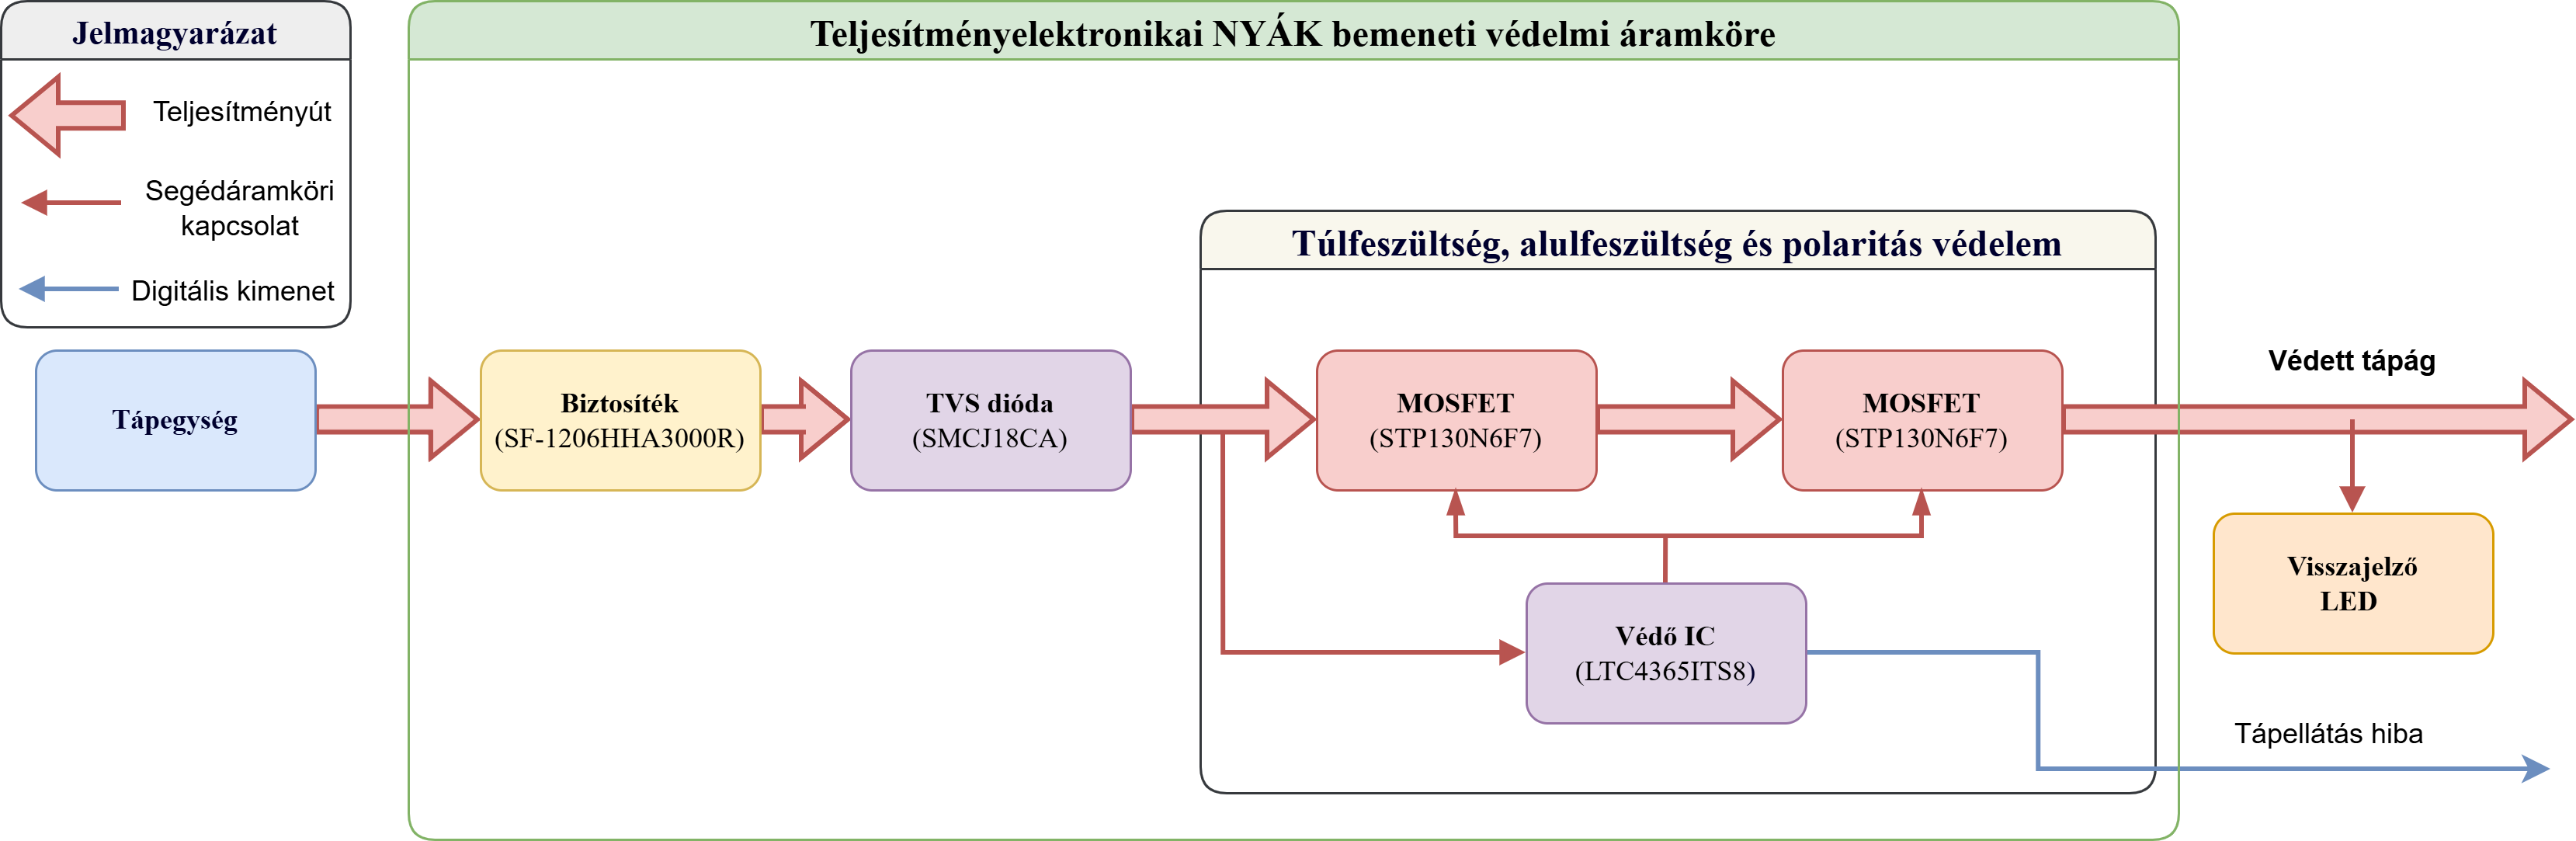
\includegraphics[width=\textwidth]{figures/Hardware/SzakdogaSystemDiagramms-PCSU_Tápvédelem.drawio.png}
    \caption{A bemeneti tápellátás védelmi egységeinek blokkvázlata}
    \label{fig:bemeneti-vedelem-blokkvazlat}
\end{figure}

\subsubsection{Túláramvédelem}
A bemeneti tápágba egy SF-1206HHA300R típusú biztosíték került
beépítésre, amely 30~A névleges áramot kibír és 50~VDC egyenfeszültségbe is alkalmazható \cite{sf-1206}.
Feladata a tápellátás megszakítása rövidzár esetén így védve a teljesítményelektronikai áramkört és a motorokat. \\

A magas névleges áram lehetővé teszi, hogy a rendszer tervezett maximális áramfelvételét \textcolor{red}{LINK}
valamint a motork indításakor fellépő áramcsúcsok (\ref{tab:motor-parameterek}) ne szakítság meg a tápellátást, azonban rövidzár
esetén a biztosíték megszakítsa a tápellátást. \\

A motorok tartós túlterhelésének és blokkolásának kezelését a motorvezérlők áramkorlátozása,
vakamint a mért motoráram szoftveres felügyelete biztosítja, nem a biztosíték megszakítása 
\textcolor{red}{LINK}.

\subsubsection{Alul és túlfeszültség és polaritás védelem}
A bemeneti tápfeszültség védelmét a NYÁK-on egy TVS dióda és egy külső MOSFET-eket vezérlő IC biztosítja. \\

A rövid idejű feszültségtranziensek korlátozására SMCJ18A típusú \cite{smcj18}, kétirányú TVS diódát alkalmaztam. 
Ezt a védelmet mint kiegészitő védelmet helyeztem az IC mellé, mely használatát a gyártó is javasolja adott 
felhasználási esetben \cite{ltc4365}.

A kiválasztott dióda záróirányú üzemi feszültsége 18~V, letörési feszültségtartomán pedig 20--22,1~V. 
Megengedett impulzus impulzus csúcsteljesítménye 1500~W  10/1000~$\mu$s impulzusforma mellett.

A kétirányú kivitel lehetővé teszi a fordított polaritás elleni védelem megtartását.
\textcolor{red}{Kicsit bullshit reason, bele kene rakni kisebbet}
\textcolor{red}{Ez helyette?} %https://hu.mouser.com/en/ProductDetail/Littelfuse/SMCJ13CA?qs=JJML70Qc14vApYMDk76Bmg%3D%3D}
\\

A bemeneti alul- és túlfeszültség, valamint a fordított polaritás elleni 
védelmet az LTC4365ITS8-1 integrált áramkör biztosítja \cite{ltc4365}.

Az IC két külső, N-csatornás MOSFET-et vezérel, közös source csatlakoztatással, 
így biztosítva a polaritás védelmet. A szembefordított testdiódák kikapcsolt állapotban mindkét irányba blokkolják a táputat, 
így megvalósítva ezt a védelmet.

Az alul és túlfeszültségvédelmi kapcsolási küszöböket 3 ellenállásból álló feszültségosztóval
segítségével állítható.  Az IC a feszültségeit az UV és OV bemenetein keresztül felügyeli,
amennyiben a tápfeszültség a megengedett tartományon kívül esik a vezérlő kikapcsolja a MOSFET-eket
így megszakítva az áramutat, és ezzel védve a teljesítményelektronikai áramkört és a motorokat. 
A hibafeltétel megszűnését követően a helyreállítási idő 
letelte után az áramkör újra engedélyezi a MOSFET-eket, így helyreállítva a tápellátást.

Az IC aktív alacsony FAULT kimenete jelzi a letiltott állapotot a mikrovezérlő felé. \\

A MOSFET-ek kiválasztásakpr a fő szempontok, hogy elbírják a maximális terhelést, amelyet
23~A maximális ármban lett meghatározva 12~V-on\textcolor{red}{LINK}.
A kiválasztott MOSFET-ek a STP130N6F7 \cite{stp130n6f7} típusúak, amelyek 
amelyek drain--source feszültsége 60~V, adatalap szerintfi folyamatos drain áramuk
pedig 80~A szobahőmérsékleten.  Az alkalmazás áramterhelhetőségének ellenőrzéséhez a vezetésgi vesztegéket és ebből
eredő üzemi hőmérséklet-emelekedést majd ennek a hatását a működésre is figyelembe lett véve. \\


A MOSFET-ek vezetési ellenállás $R_{\mathrm{DS(on)}}$ értéke 5.0~m$\Omega$, 
amely a meghatározott 23~A maximális terhelés mellett \textcolor{red}{LINK} MOSFET-enkénti teljesítményvesztesége:\\
\begin{equation}
    \label{eq:vedelem-mosfet-veszteseg}
    P_{\mathrm{Q}} = I_{\mathrm{max}}^2 R_{\mathrm{DS(on)}}
    = (23~\mathrm{A})^2\cdot5{,}0~\mathrm{m}\Omega
    \approx2{,}65~\mathrm{W}.
\end{equation}
Az adatlap alapján a MOSFET-ek $R_{\theta\mathrm{JA}}=62{,}5$~K/W hőellenállással rendelkeznek. Az \eqref{eq:vedelem-mosfet-veszteseg} 
egyenlet szerinti veszteséggel számított hőmérséklet-emelkedés:
\begin{equation}
    \label{eq:vedelem-mosfet-homersekletemelkedes}
    \Delta T_{\mathrm{J}} = P_{\mathrm{Q}} R_{\theta\mathrm{JA}}
    \approx2{,}65~\mathrm{W}\cdot62{,}5~\mathrm{K/W}
    \approx165{,}6~\mathrm{K}.
\end{equation}
Ez 25~$^\circ$C környezeti hőmérséklet mellett 190.6~$^\circ$C csomóponti hőmérsékletet eredményez. 
Ez meghaladja a megengedett maximális hőmérsékleti határértékét a MOSFET-eknek 175~$^\circ$C, 
így hűtőbordák alkalmazása szükésges. \\

A hűtés méretezéséhez maximális 40 fokos környezeti hőmérséklet és maximális 100 fokos csomóponti hőmérsékletre lett méretezve. 
A MOSFETek vezetési ellenállása 100$^\circ$C fokon az adatlabból kiolvas 8 m$\Omega$-nak felel meg, így a teljesítményveszteség
egy MOSFET-en:
\begin{equation}
    \label{eq:vedelem-mosfet-meleg-veszteseg}
    P_{\mathrm{Q,100}} = I_{\mathrm{max}}^2 R_{\mathrm{DS(on)}}(100~^\circ\mathrm{C})
    = (23~\mathrm{A})^2\cdot8~\mathrm{m}\Omega
    \approx4{,}23~\mathrm{W}.
\end{equation}

Ebből a megengedett teljes csomóponti--környezeti hőellenállás:
\begin{equation}
    \label{eq:vedelem-megengedett-hoellenallas}
    R_{\theta\mathrm{JA,max}}
    =\frac{T_{\mathrm{J,cel}}-T_{\mathrm{A,max}}}{P_{\mathrm{Q,100}}}
    =\frac{(100-40)~\mathrm{K}}{4{,}23~\mathrm{W}}
    \approx14{,}2~\mathrm{K/W}.
\end{equation}

A teljes hőút a csomópont--tok, a tok--hűtőborda és a hűtőborda--környezet hőellenállásból áll.
Így a hűtőborda megengedett hőellenállása külön hűtőborda alkalmazása esetén:
\begin{equation}
    \label{eq:vedelem-hutoborda}
    R_{\theta\mathrm{SA}}
    \leq R_{\theta\mathrm{JA,max}}
       -R_{\theta\mathrm{JC}}
       -R_{\theta\mathrm{CS}}
    = 13{,}26~\mathrm{K/W}
       -R_{\theta\mathrm{CS}}.
\end{equation}
Ahol az $R_{\theta\mathrm{CS}}$ a tok--hűtőborda hőellenállása, ami a hűtőborda rögzítésének módjától függően változik.

\textcolor{red}{Hűtőborda választás?} \\

A 23~A-es méretezési áram a rendszer fennálható legnagyobb egyidejű terhelését jelenti, amely
üzemszerűen csak rövid ideig állhat fenn. A hűtés előzetes méretezése során ezt az áramot
tartósnak feltételeztem, konzervatív becslést adva a szükséges hőelvezetésre.
A tényleges üzemi hőmérsékletet terheléses méréssel szükséges ellenőrizni, és
a mért értékből számítani a szükséges hőelvezetést.

\subsubsection{Kimeneti túlfeszültség védelem}
\textcolor{red}{EZT MEG MEG KEKL TERVEZNI}

\subsubsection{Motor visszatáplalási elleni védelem}
\textcolor{red}{EZT MEG MEG KEKL TERVEZNI}

\subsubsection{Kapcsolási rajz}
A bemeneti védelem kapcsolási rajzát a \ref{fig:bemeneti-tapellatas-vedelem-rajz}.~ábra
mutatja be. Az F1 biztosítékot a bemeneti tápágba sorosan kapcsoltam. A D5 TVS-dióda a biztosíték
utáni csomópont és a GNDPWR földhálózat közé csatlakozik.

Az LTC4365ITS8-hoz áramköri kialakítása a gyártói adatlap [14.]~ábráját vette alapul. 
Az R14-es ellnállását az aktív alacsony SHDN bemenetet a bemeneti tápfeszültséghez
lett kapcsolva, így a vezérlő normál tápellátás mellett engedélyezi. A BAT\_FAIL jel a FAULT 
kimeneti állapotát továbbítja a központi vezérlőpanel felé. A sikeres működés után a védett 12~V-os ágon
LED ad visszajelzést ad a felhasználó számára. \\


A MOSFET-ek kapujához egy-egy 10ˇ$\omega$-os soros ellenállás, R15 és R16 kapcsolódik.
A bekapcsolási feszültségfelfutatás lassítását a GATE kimenet és a föld közé kapcsolt R17
és C16 alkotta soros ág biztosítja. A védett kimeneti tápágon a C17-es 100~$\mu$F mérsékeli
a bekapcsoláskor fellépő áramlökést. \\


Az alul és túlfeszültségi kapcsolási küszöböket a feszültségosztó R11, R12 és R13
ellenállások határozzák meg.
Az ellenállások méretezésekor figyelembe kell venni az UV bemenet 
szivárgási áramát. Az adatlap szerint a legrosszabb szivárgási áram $I_{\mathrm{UV,max}}$ értéke 10~nA.
A gyártó méretezését követve a szivárgóáram okozta megengedett feszültséghiba 
($V_{\mathrm{hiba,max}}$) értékére használt 3~mV-os érték lett alapul véve.
Ezek az alsó két ellenállás összehének felső határa:
\begin{equation}
R_{12}+R_{13}
    \leq\dfrac{V_{\mathrm{hiba,max}}}{I_{\mathrm{UV,max}}} =\dfrac{3~\mathrm{mV}}{10~\mathrm{nA}}
    =300~\mathrm{k}\Omega.
    \label{eq:vedelem-oszto-hibakeret}
\end{equation}

Alulfeszültségi határ beállításához a következő képletet kell alkalmazni, ahol 
$V_{\mathrm{UV}}$ az alulfeszültségi lekapcsolási küszöb, amelyet 8~V-ban lett meghatározva, 
$V_{\mathrm{REF}}=0{,}5$~V pedig az IC névleges komparátorküszöbe. 
Az \eqref{eq:vedelem-oszto-hibakeret} alapján 300~k$\Omega$ ellenállásösszeget választva:
\begin{equation}
    R_{11}
    =(R_{12}+R_{13})\frac{V_{\mathrm{UV}}-V_{\mathrm{REF}}}{V_{\mathrm{REF}}}
    =300~\mathrm{k}\Omega\cdot\frac{8-0{,}5}{0{,}5}
    =4{,}5~\mathrm{M}\Omega.
    \label{eq:vedelem-r11}
\end{equation}

A túlfeszültségi lekapcsolási küszöböt $V_{\mathrm{OV}}=15$~V értékben lett meghatározva. 
Az ehhez szükséges R13 ellenállás értéke a következőképpen számítható:
\begin{equation}
    R_{13}
    =\frac{V_{\mathrm{REF}}}{V_{\mathrm{OV}}}(R_{11}+R_{12}+R_{13})
    =\frac{0{,}5}{15}\cdot4800~\mathrm{k}\Omega
    =160~\mathrm{k}\Omega.
    \label{eq:vedelem-r13}
\end{equation}

Az R12-es ellenállás értéke a\eqref{eq:vedelem-oszto-hibakeret} egyenlethez választott összegből 
és az \eqref{eq:vedelem-r13} eredményéből számítható:
\begin{equation}
    R_{12} = (R_{12}+R_{13})-R_{13}
    =(300-160)~\mathrm{k}\Omega=140~\mathrm{k}\Omega.
    \label{eq:vedelem-r12}
\end{equation}

\textcolor{red}{Miert 8 és 15 V a levagasi fesz?? - erre vmi jobb indokot talalni; vagy ha nem
atmeretezni 3S Li-ion akksira: ott a levagasi fesz 9 a felso meg ~13V (esetleg 14V)}

A bekapcsoláskor keletkező áramlökés az IC GATE kimenetéhez az R17
ellenálláson keresztül C16 kondenzátor mérsékeli. 
Bekapcsoláskor az IC névleges 20~$\mu$A áramot biztosít a GATE bemenetekre.
A gártói adatalap közelítésével a kiemeneti feszültségi meredeksége a következő képlettel számítható ki:
\begin{equation}
    s_{\mathrm{OUT}}=\frac{\Delta V_{\mathrm{OUT}}}{\Delta t} \approx \frac{I_\mathrm{GATE}}{C_{16}}
    = \frac{20\cdot10^{-6}}{10\cdot10^{-9}}
    = 2~\mathrm{V/ms}.
    \label{eq:vedelem-felfutasi-meredekseg}
\end{equation}
Az ehhez tartozó kapacitív töltési áram:
\begin{equation}
    I_{\mathrm{inrush}}=C_{\mathrm{OUT,ossz}}s_{\mathrm{OUT}}
    \approx\frac{C_{\mathrm{OUT,ossz}}}{C_{16}}I_{\mathrm{GATE}}.
    \label{eq:vedelem-inrush-altalanos}
\end{equation}
ahol $C_{\mathrm{OUT,ossz}}$ a védett 12~V-os ágra közvetlenül kapcsolódó kondenzátorok összesített kapacitása.

Ez az érték becsülhető a bemeneti védő IC-hez kapcsolt 100~$\mu$F 
és a motorvezérlőkhöz tartozó 2~db 470~$\mu$F-os kondenzátor összegeként. \\
Az \eqref{eq:vedelem-inrush-altalanos} egyenletbe helyettesítve ezt a 1040~$\mu$F-os összeget:
\begin{equation}
    I_{\mathrm{inrush}}
    \approx\frac{(100+2\cdot470)\cdot10^{-6}~\mathrm{F}}{10\cdot10^{-9}~\mathrm{F}}
    \cdot20\cdot10^{-6}~\mathrm{A}
    =2{,}08~\mathrm{A}.
    \label{eq:vedelem-inrush-becsles}
\end{equation}

A névleges kaputöltő árammal becsült felfutási idő 15~V-os bemenetnél, az \eqref{eq:vedelem-felfutasi-meredekseg} alapján:
\begin{equation}
    t_\mathrm{rise}
    = \frac{V_{\mathrm{IN,max}}}{s_{\mathrm{OUT}}}
    = \frac{15}{2}
    \approx 7{,}5~\mathrm{ms}.
    \label{eq:vedelem-felfutasi-ido}
\end{equation}

A bekapcsolási terhelés becsléséhez az \eqref{eq:vedelem-inrush-becsles} szerinti 2,08~A-es töltőáramot és az \eqref{eq:vedelem-felfutasi-ido} szerinti 7,5~ms-os felfutási időt vettem alapul 15~V bemeneti feszültség mellett.
Az adatllapban elérhető adatait a bekapcsolás során aMOSFET-nek folytonos 15~V-os feszültséget feltételeztem 
és 10~ms-os impulzushoz tartozó határgörbéről hozzávetőlegesen 10~A-es megengedett áram 
olvasható le, így a számított munkapont a biztonságos működési tartományban helyezkedik el.
Az ellenőrzés 25~$^\circ$C környezeti hőmérséklet, egyszeri bekapcsolásra és a kimeneti kondenzátorok
feltöltésére vonatkozik. 

\begin{figure}[H]
    \centering
    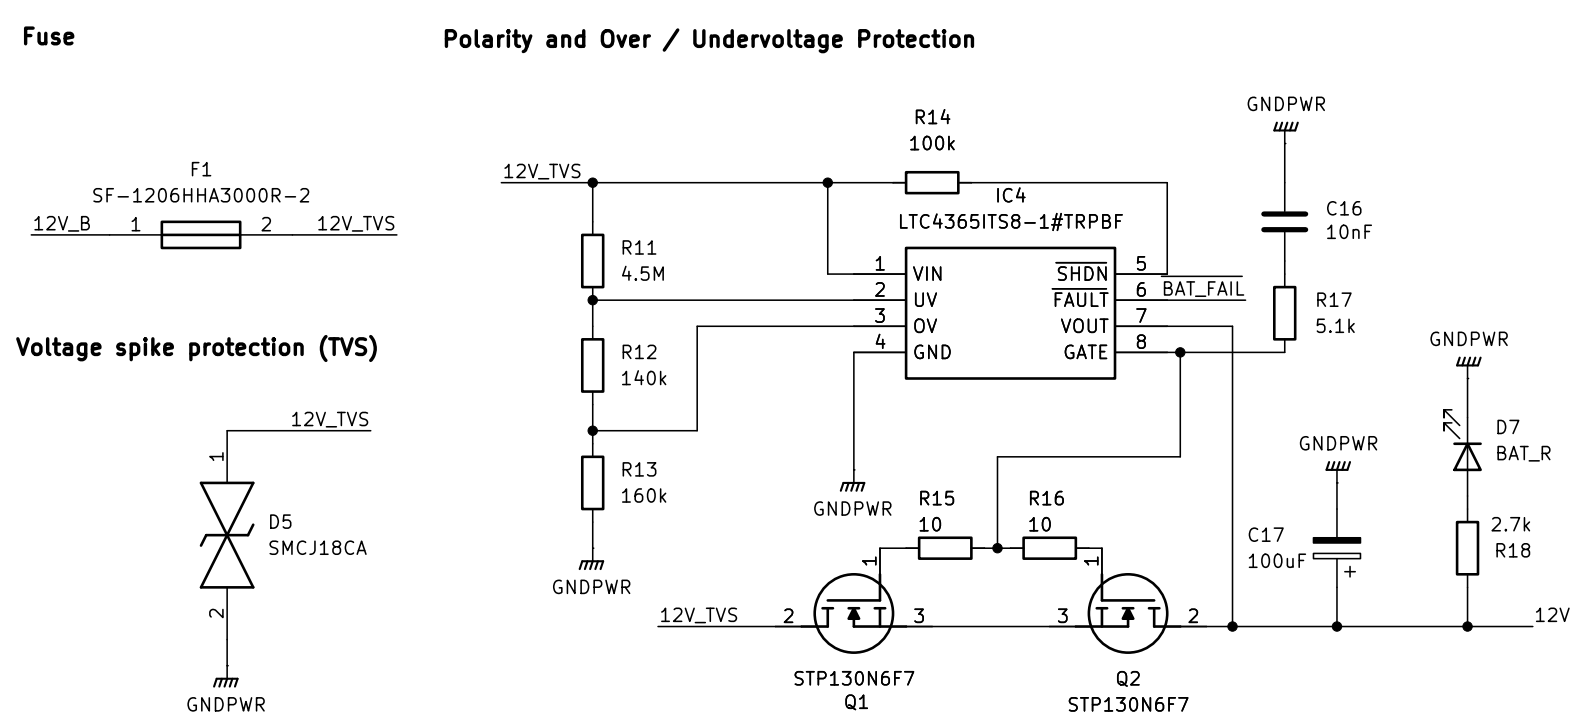
\includegraphics[width=\textwidth]{figures/Hardware/Battery_Prot_PCSU_Schematic.png}
    \caption{A bemeneti tápellátásvédelem kapcsolási rajza}
    \label{fig:bemeneti-tapellatas-vedelem-rajz}
\end{figure}

\subsubsection{Huzalozási terv}
A bemeneti védelmi áramkört a tápkacsolás közelében helyezkedik el.
Az egy területre történő csoportosítás lehetővé teszi a bemeneti áramút rövid kialakítását.
Széles vezetősávok és rézkitöltések biztosítják az összeköttetéseket, ezzel csökkentve a
vezetési ellenállást és abból eredő feszültségesést. Emellett pedig a megfelelő hőelosztást is 
segítik az alkatrészek számra. \\

A TVS-diódát a bemeneti csatlakozó és a biztosíték közelében helyeztem el. 
A tápág és a földhálózatközötti csatlakozásait rövidre alakítottam,
így mérsékelve a parazita induktivitás hatását a tranzienskorlátozásra. \\

Az LTC4365 vezérlőhöz tartozó elemeket az elrendezését a gyártó altal javasolt szempontok alapján lett kialakítva \cite{ltc4365}. 
A MOSFET-eket a vezérlő közelében helyezezkednek el, és tajolásuk olyan,
hogy a hozzájuk tartozó hűtőbordák a panel azonos oldala felé helyezkedhessenek el. 
Az áramlökést korlátozó C16 kondenzátort az IC-hez közelében kapott helyett. A pufferkondenzátor a MOSFET-ek 
közvetlen közelében került elhelyezésre.

\textcolor{red}{kellett vna kis kondi ide a datasheet szerint (ajánlott)}

\begin{figure}[H]
    \centering
    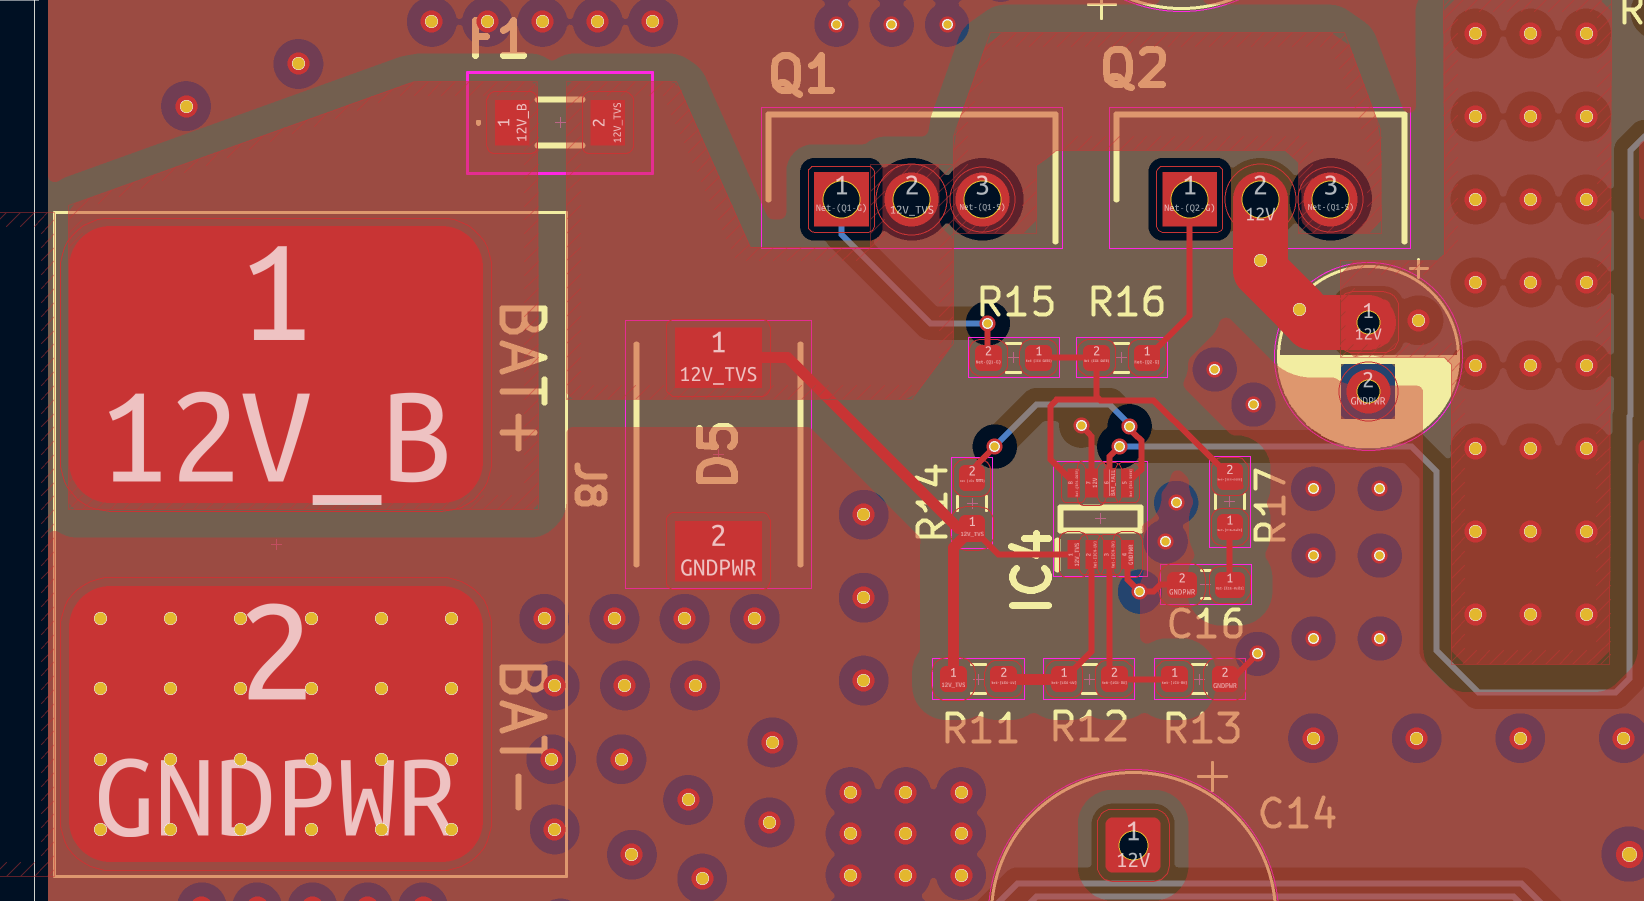
\includegraphics[width=0.8\textwidth]{figures/Hardware/Battery_Prot_PCSU_PCB.png}
    \caption{A bemeneti tápellátásvédelem huzalozási terve}
    \label{fig:bemeneti-tapellatas-vedelem-huzalozasi-terv}
\end{figure}




\subsection{5V-os tápfeszültség előálltása}
A vezérlőpanel tápellátásához szükséges 5~V-os feszültséga 12~V-os
bemeneti tápfeszültségből egy TPS54628 szinkron buck konverter segítségével
állítja elő \cite{tps54628}.
Az integrált áramkör 4.5--18~V bemeneti feszültségtartományba használható és
0.76--5.5~V-ig kimeneti feszültséget képes előállítani. Legfeljebb
6~A áram biztosítására alkalmas, ami a vezérlőpanel várható terheléséhez képest
jelentős tartalékot tesz lehetővé \textcolor{red}{LINK}.

\subsubsection{Kapcsolási rajz}
A buck konverter kapcsolási bekötésének kialakítási alapját a gyártói 
[8.2]~ alfejezetében bemutatott tipikus alkalmazás valamint az [1. Table] megadott
alkatrészek és értékeik adták \cite{tps54628}. A megvalósított kapcsolást a
\ref{fig:buck-konverter-kapcsolasi-rajz}. ~ábra mutatja be.

Az EN engedélyező bemenet az R3 ellenálláson keresztül a bemeneti
tápfeszültséghez van kötve, így a konverter mindig aktív üzenmódban van
a tápellátás bekapcsolását követően. A kimeneti feszültséget az R1 és 
R2 ellenállásolból álló visszacsatolás osztó határozza meg. A D1 LED és 
az R5 előtét ellenállás az 5~V-os  tápág feszültségét jelzi a felhasnáló számára.

A tekercs méretezésénél figyelembe lett véve az azon folyó áram 
csúcsérte és effektív értéke. 
A gyártó az induktivitás áramának csúcstól csúcsig mért hullámosságára
a következő képletet adta meg \cite{tps54628}: 
\begin{equation}
    \Delta I_{\mathrm{L}} = \frac{V_{\mathrm{OUT}}}{V_{\mathrm{IN}}}
    \frac{V_{\mathrm{IN}}-V_{\mathrm{OUT}}}{L f_{\mathrm{SW}}}.
    \label{eq:buck-aramhullamossag}
\end{equation}
ahol $L$ az induktivitás értéke, $f_\mathrm{SW}$ pedig a kapcsolási frekvencia.
A névleges 12~V-os bemeneti és 5~V-os kimeneti feszültség,
3{,}3~$\mu$H induktivitás és 650~kHz kapcsolási frekvencia
mellett az \eqref{eq:buck-aramhullamossag} alapján:
\begin{equation}
    \Delta I_{\mathrm{L}} = \frac{5}{12}\frac{12-5}{3{,}3\cdot10^{-6}\cdot650000}
    \approx1{,}36~\mathrm{A}.
    \label{eq:buck-aramhullamossag-ertek}
\end{equation}

Így az induktivitás áramának csúcsértéke 5~A-es maximális
kimeneti terhelés a következő:
\begin{equation}
    I_{\mathrm{L,peak}}=I_{\mathrm{OUT}}+\frac{\Delta I_{\mathrm{L}}}{2}
    =\left(5+\frac{1{,}36}{2}\right)~\mathrm{A}
    \approx5{,}68~\mathrm{A}.
    \label{eq:buck-csucsaram}
\end{equation}

Háromszög alakú hullámosságot feltételezve, az induktivitáson folyó áram effektív értéke a következő:
\begin{equation}
    I_{\mathrm{L,RMS}}=\sqrt{I_{\mathrm{OUT}}^2+\frac{\Delta I_{\mathrm{L}}^2}{12}}
    =\sqrt{5^2+\frac{1{,}36^2}{12}}~\mathrm{A}
    \approx5{,}02~\mathrm{A}.
    \label{eq:buck-effektiv-aram}
\end{equation}

A kiválasztott induktivitás névleges áramterhelhetősége
6~A, telítési árama pedig 12~A~\cite{BMRA000606303R3MA1}.
A \eqref{eq:buck-effektiv-aram} szerinti effektív áramérték a névleges
áramterhelhetősége alatt marad, az \eqref{eq:buck-csucsaram} szerinti csúcsáram pedig jelentősen kisebb a telítési áramnál.

\begin{figure}[H]
    \centering
    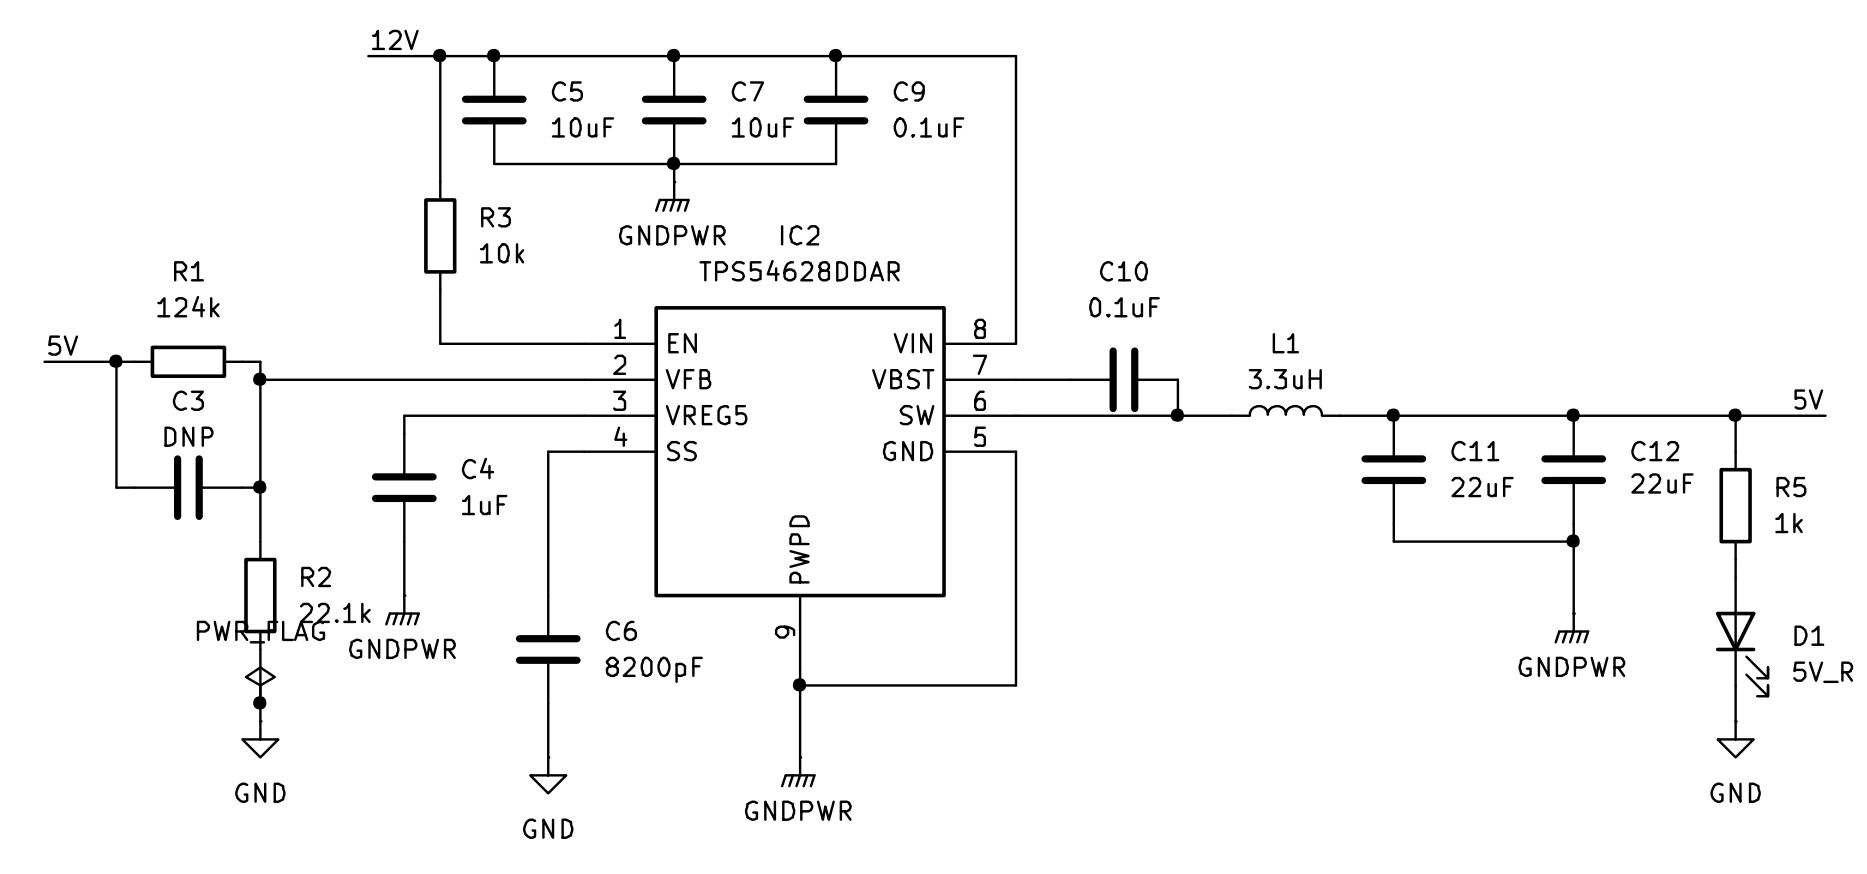
\includegraphics[width=\textwidth]{figures/Hardware/Buck_Converter_Schematic.png}
    \caption{TPS54628 buck konverter kapcsolási rajza}
    \label{fig:buck-konverter-kapcsolasi-rajz}
\end{figure}

\subsubsection{Huzalozási terv}
A konverter huzalozási terve követte a gyártói adatlapban [10.1]~alfejezben levő irányelvek
és a [10.2]~alfejezetben bemutatott áramköri kialakítást \cite{tps54628}. 

A bemeneti szűrőkondenzátorak az IC-hez minnél közelebbi elhelyezését,
így csökkentve a kapcsolási áramhurkokat. Emellett a teljesítményágban minnél szélesebb rézfelületek alkalmazását,
a vezetési ellenállás és parazita induktivitás csökkentésére, valamint a hővezetés segítéséhez.
Az IC középső hővezető padját viákon keresztül további földrétegekhez kapcsolódva segíti az IC
hőelvezetését. A nagyteljesítmenyű GNDPWR földhálózatból, a visszacsatoló és 
lágyindító kondenzátorok GND visszavezetését, valamint az 5~V-os fogyasztók
földhálózatát egy pontból lettek visszavezetve, így elkerülve a földhurok kialakulását. \\

\textcolor{red}{Kisebb földmenet az L1-hez így nagyobb a zavar? (kondiig biztosan)}
\textcolor{red}{ezzel biztosan elkeruli a foldhurkot?}
\textcolor{red}{mashol kellett vna leveztnem a 5V groundot? javitani a PCB-t}

\begin{figure}[H]
    \centering
    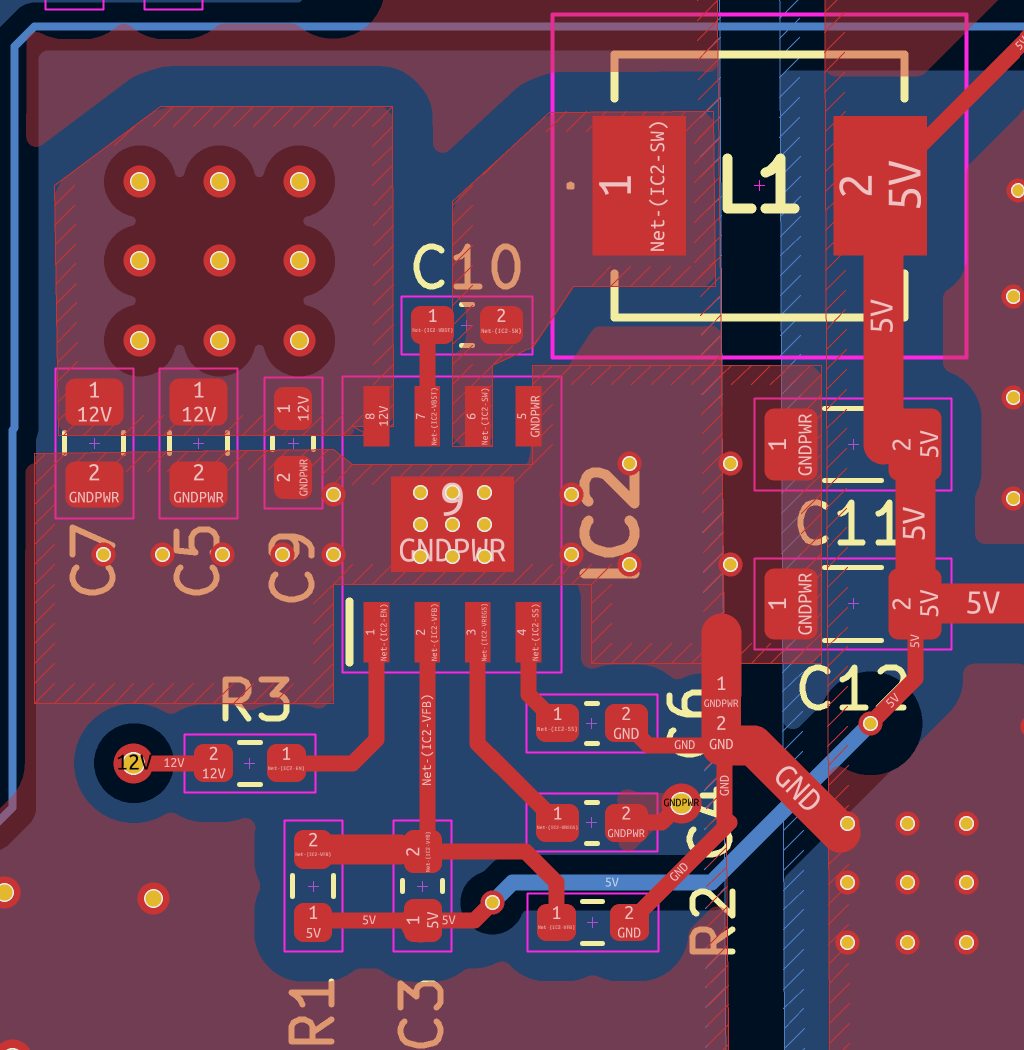
\includegraphics[width=0.7\textwidth]{figures/Hardware/Buck_Converter_PCB.png}
    \caption{TPS54628 buck konverter huzalozási rajza}
    \label{fig:buck-konverter-huzalozasi-rajz}
\end{figure}

\subsection{Motorvezérlés}
A két tengelynek motorjának meghajtásához a kiválasztott DRV8244SQDGQRQ1 
(\ref{subsec:motorvezerlok-kiválasztas}) típusú integrált áramkörök kerültek 
kiválasztásra \cite{drv8244}. 
A két motorvezérlő felépítése azonos és elrendezése hasonló. A meghajtók konfigurálására
és diagnosztikai adatok kiolvasását a központi vezérlőpanel SPI-on végzi.
Azonban a motork irányítását a további lábakon keresztül
történik GPIO és PWM jelek segítségével. 

\subsubsection{Kapcsolási rajz}
Az IC-k schematikja követte a gyártói adatlapban [8.3.1.2]~alfejezetben lévő
passzív alkatrész ajánlásokat és a [9.2]~alfejezetben bemutatott tipikus alkalmazás kapcsolási
rajzát \cite{drv8244}. A megvalósított áramkört
a \ref{fig:drv8244-q1-kapcsolasi-rajz}.~ábra mutatja be. \\


Az IPROPI kimenethez tartozó C8, C15 szűrő kondenzátor és R\_IP1 és R\_IP2 ellenállások 
a motorárammal arányos feszültséget biztosítanak a központi vezérlőpanel számára.
Az ellenállások méretezéséhez a gyártó által [7.5.8]-ban meghatározott osztási arányt használtam,
amellyel a következő módon számolható ki az ellenálláson megjelenő feszültség:
\begin{equation}
    V_{\mathrm{IPROPI}}=\frac{I_{\mathrm{MOTOR}}R_{\mathrm{IPROPI}}}{A_{\mathrm{IPROPI}}},
    \qquad A_{\mathrm{IPROPI}}=4570.
    \label{eq:motor-ipropi-feszultseg}
\end{equation}
Az \eqref{eq:motor-ipropi-feszultseg} alapján $R_{\mathrm{IPROPI}}$ felső határa 10~A motoráramnál és 3,3~V névleges mérési határnál:
\begin{equation}
    R_{\mathrm{IPROPI}}\leq\frac{V_{\mathrm{IPROPI,max}}A_{\mathrm{IPROPI}}}{I_{\mathrm{MOTOR,max}}}
    =\frac{3{,}3\cdot4570}{10}~\Omega
    \approx1{,}51~\mathrm{k}\Omega.
    \label{eq:motor-ipropi-ellenallas}
\end{equation}
A számított felső határnál kisebb, 1~k$\Omega$ névleges ellenállást 
választottam. Ezzel a maximum10~A motoráramnál a várható névleges IPROPI-feszültség:
\begin{equation}
    V_{\mathrm{IPROPI}}=\frac{I_{\mathrm{MOTOR}}R_{\mathrm{IPROPI}}}{A_{\mathrm{IPROPI}}}
    =\frac{10\cdot1000}{4570}~\mathrm{V}
    \approx2{,}19~\mathrm{V}.
    \label{eq:motor-ipropi-ertek}
\end{equation}
amely érték megfelelő feszültségtartalékot hagy a motoráram méréshez a mikrovezérlőn. 

Az IPROPI kimenetekhez párhuzamosan kapcsolódó C8 és C15 kondenzátorok kapacitása 100~nF, így az
1~k$\Omega$-os ellenállásokkal alkotott hálózat névleges időállandója 100~$\mu$s.

\textcolor{red}{ezt meg leosztom majd, mert lehet 5V?? - ha vmi error van... (lehet jobb lenne az 1.5k)}

Az aktív alacsony nSLEEP bemenetekhez kapcsolt R4 és R10 10~k$\Omega$-os lehúzóellenállások alacsony
szinten tartják az engedélyező jeleket, amíg a mikrovezérlő nem kezdeményezi
a meghajtók ébresztését.
Az aktív alacsony, open drain nFAULT kimenetek felhúzóellenállásai a központi
vezérlőpanelen kaptak helyet \textcolor{red}{LINK}. \\

Mindkét meghajtó tápbemenetéhez a gyártó által ajánlott, az adatlap
[10]~fejezetben alapján a 100~nF-oskerámai szűrőkondenzátort, valamint 470~uF-ospuffferkondenzátor lett kapcsolva 
\cite{drv8244}. A választott pufferkapacitás megfelelőségét a motorok terhelés alatti 
indításakor és fékezésekor végzett tápfeszültségméréssel
szükséges ellenőrizni, a feszültségesések és túlfeszültségek vizsgálatával.

\textcolor{red}{Méréssel validálni kell} 

\begin{figure}[H]
    \centering
    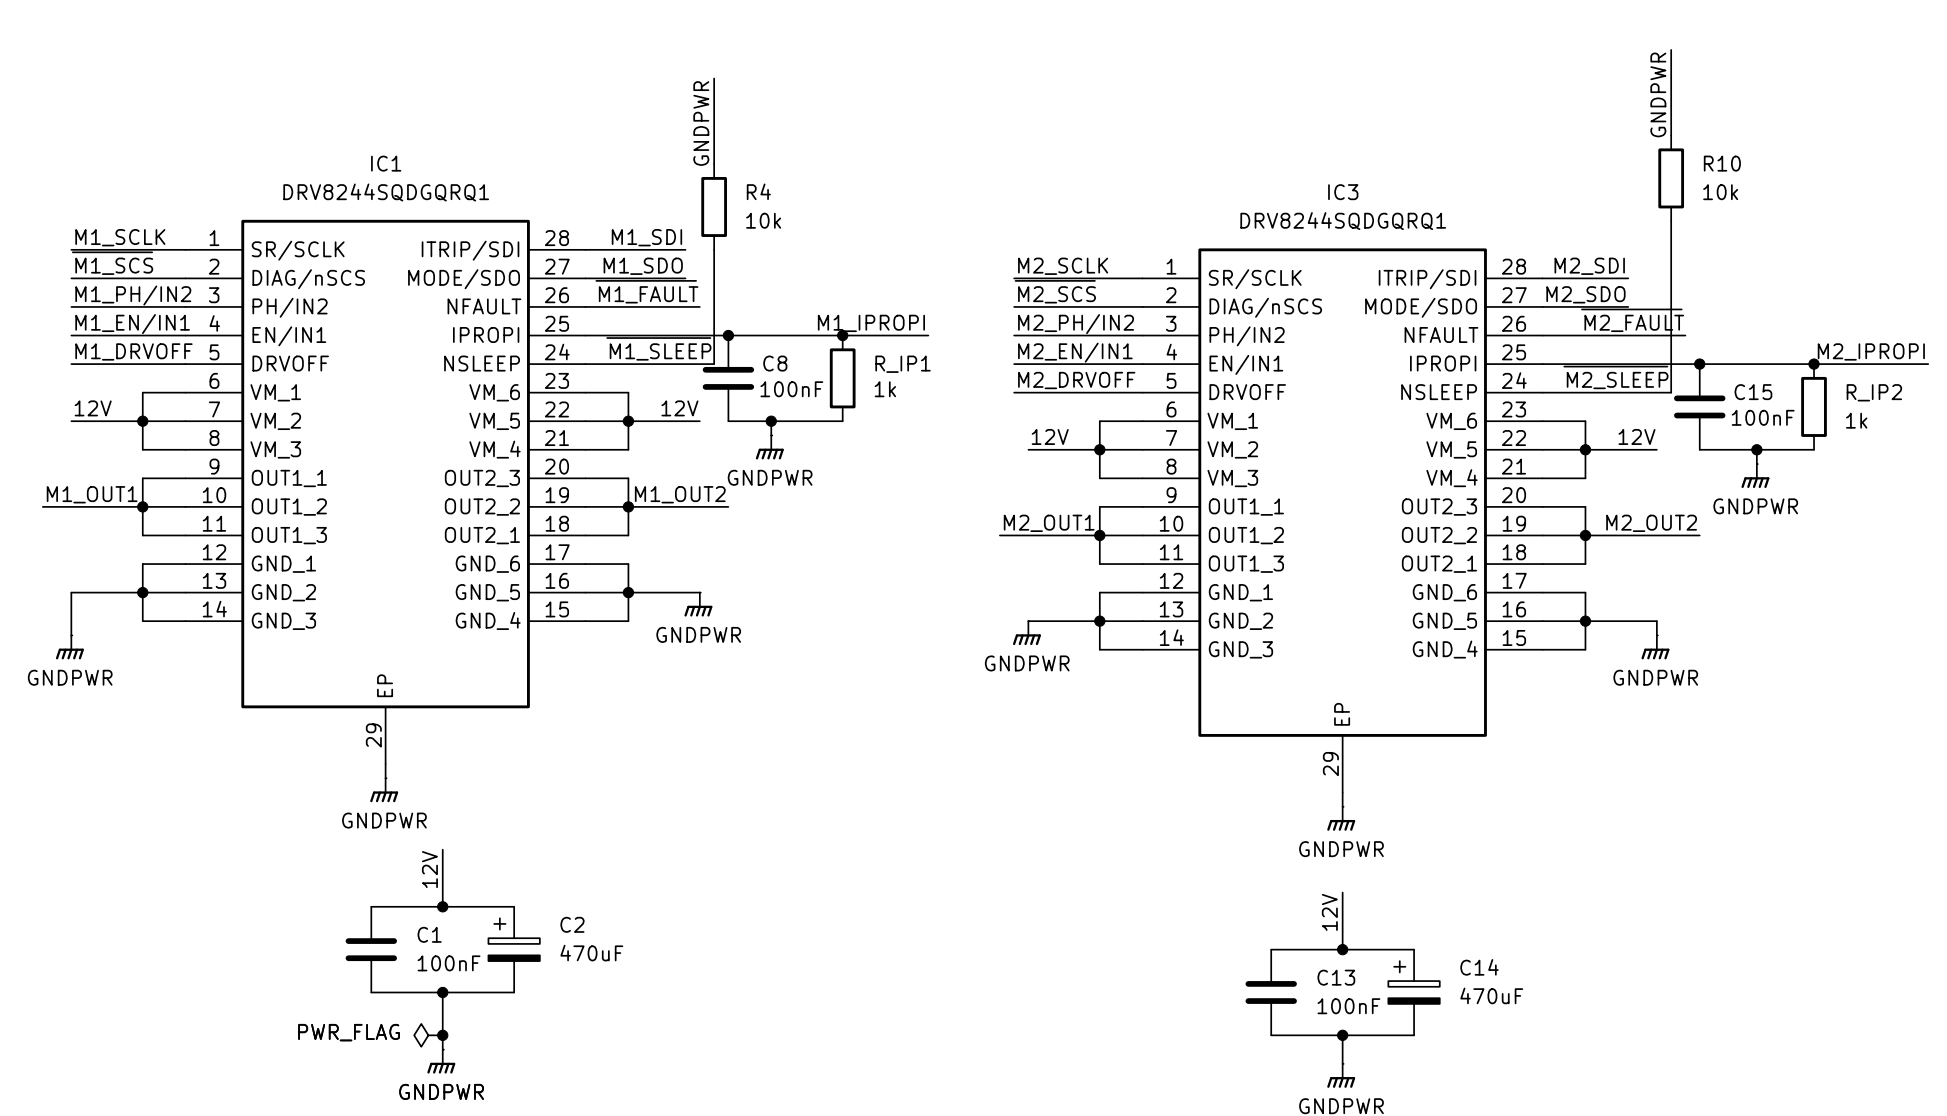
\includegraphics[width=\textwidth]{figures/Hardware/MotorController_Schematic.png}
    \caption{DRV8244-Q1 motorvezérlők kapcsolási rajza}
    \label{fig:drv8244-q1-kapcsolasi-rajz}
\end{figure}


\subsubsection{Huzalozási terv}
A motorvezérlők huzalozási terve a gyártói [11]~fejezetében található
irányelveket és bemutatott tipikus alkalmazás huzalozási tervét figyelembe véve készült \cite{drv8244}. 

A 100~nF-os kerámia szűrökondenzátorok az IC-k tápbemenetéhez közel lettek elhelyezve,
valamint pufferkondenzátorok szintúgy a motorvezérlőkhöz kozel kaptak helyet.  

A táp és motorkimeneti ágak széles vezetősávokkal és rézkitöltéssel
lettek kialakítva, így csökkentve a vezetési ellenállást és az abból adodó feszültségesést. 
Az IC központi hővezető padja és környezete viákon keresztül további földrétegekhez kapcsolódik, így
segítve a hőelvezetést. \\

Az IPROPI mérőjeleinek vezetésénél kerülve volt a kapcsolóüzemű motorkimenetek közvetlen
közelségét, a zavarcsatolás mérséklése érdekében.

\textcolor{red}{vitatható ez a közelség azért némileg}
\textcolor{red}{Itt sem biztos h a legjobbak a kitolteseim + tobb via kellett vna}

\begin{figure}[H]
    \centering
    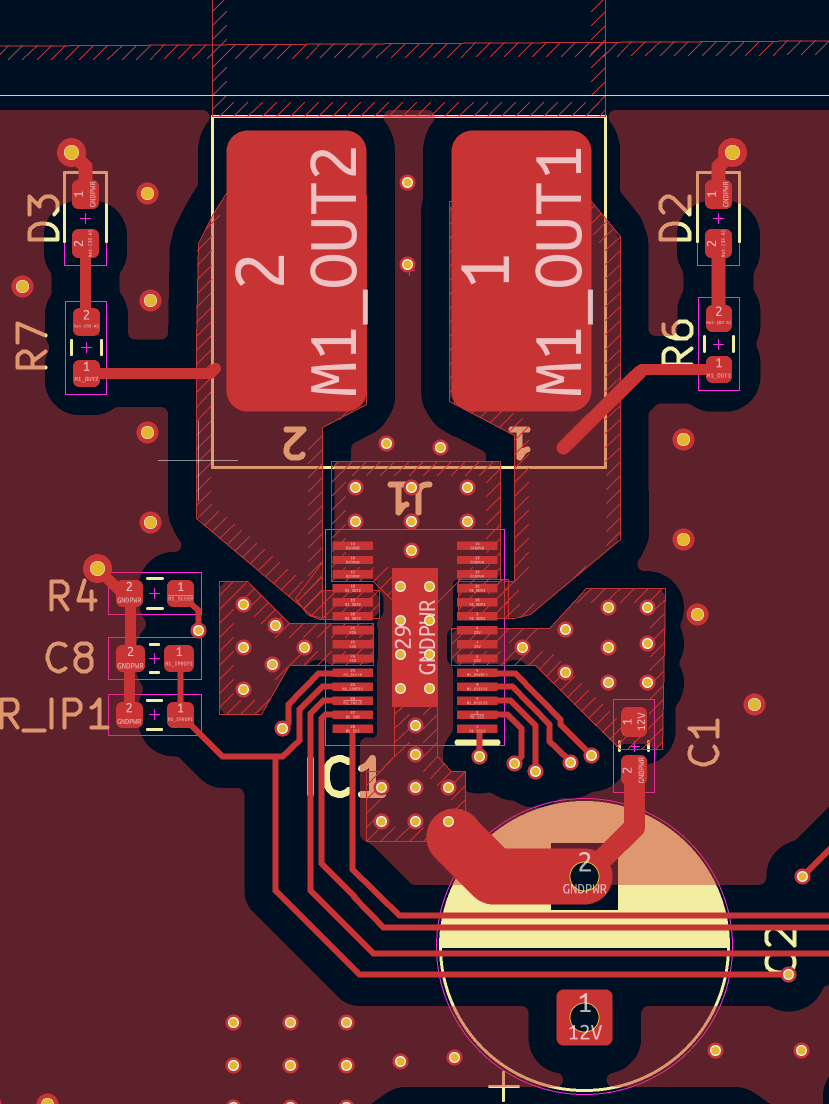
\includegraphics[width=0.48\textwidth]{figures/Hardware/MotorController_PCB1.png}
    \hfill
    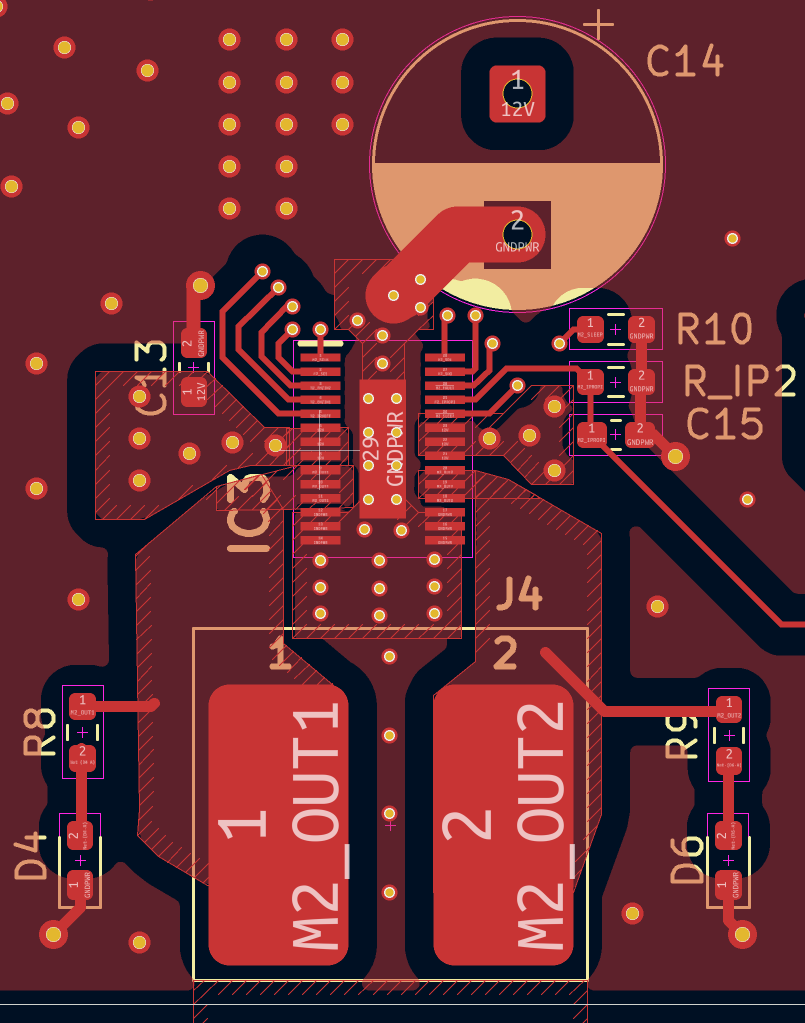
\includegraphics[width=0.48\textwidth]{figures/Hardware/MotorController_PCB2.png}
    \caption{A DRV8244-Q1 motorvezérlők huzalozási rajza}
    \label{fig:drv8244-q1-huzalozasi-rajz}
\end{figure}

\subsection{Vezérlőjelek, áram visszacsatolás és állapotjelzők}
A teljesítményelektronikai panel és a központi vezérlőpanel közötti
csatlakozások biztosítják az 5~V-os tápellátást, a motorvezérlő
jelek továbbítását, valamint a mérési és hibajelzések visszavezetését.
A tápágak és a motorkimenetek állapotának vizuális visszahelzésére
a panelen elhelyezett LED-ek segítik.

\subsubsection{Bemeneti tápfeszültség mérése}

A panelen egy feszültségosztó biztosítja a már védett 12~V-os tápfeszültség visszacsatolását a központi vezérlőpanel számára.
Az R19-es ellenállás 100~k$\Omega$-os, az R20-as ellenállás pedig 18~k$\Omega$-os ami a GND-hez kapcsolódik
így az átvitt feszültség a maximum 15~V esetén:
\begin{equation}
    V_{\mathrm{BAT,ADC}}=V_{\mathrm{IN}}\frac{R_{20}}{R_{19}+R_{20}}
    =15\frac{18}{100+18}~\mathrm{V}
    \approx2{,}29~\mathrm{V}.
    \label{eq:vedelem-feszultseg-osztas}
\end{equation}

\subsubsection{Csatlakozók}
A bemeneti tápvezeték és a motorvezetékek közvetlenül 
NYÁK felületén kialakított forrasztópadokhoz csatlakoznak. A kialakítás
lehetővé teszi a vezetékek párhuzamos elvezetését. A kapcsolat bonthatóságát
a kábeleken lévő csatlakozók biztosítják. A bemeneti akkumlátorhoz egy XT30-as 
csatlakozó tartozik, míg a motorvezetékek csatalakozóinak 
típusa a motorokon található JST csatlakozókhoz igazódik.

\textcolor{red}{Motoroknal azrtt JST mert maga a motor is JST csatis..}
\textcolor{red}{Ezt átcserélni csatira?} \\

Az 5~V-os tápellátás biztosítását és a tápellátáshoz kapcsolódó jelekhez a központi vezérlőpanelhez egy 6 pólusú
JST csatlakozó tartozik. Ezkeből 2~db az 5~V-os tápághoz és 2~db az 5~V földhálózatához 
csatlakozik. Ennek célja, hogy egy csatlakozóra jutó áramterhelést csökkentse, mivel a JST
csatlakozó maximális áramterhelhetősége 3~A, így az 5~V-nak \textcolor{red}{LINK} a maximális terheléséhez 2--2 csatlakozás
szükséges \textcolor{red}{datasheet}. 

A maradék 2 értinkező a bemeneti bédelmi áramkör hibakimenete és a védett 12~V-os tápág 
feszültségével arányos analóg mérőjelet továbbítja a vezérlőpanel felé. \\

A két motorvezérlőhöz külön SPI- és vezérlőcsatlakozó tartozik.
Az SPI-csatlakozó a konfigurációhoz és az állapotadatok
kiolvasásához szükséges jeleket vezeti ki, míg a  vezérlőcsatlakozón a motor működtetéséhez szükséges
vezérlőjelek, a hibajelzés és az árammal arányos IPROPI analóg 
feszültség visszacsatolása található.

\textcolor{red}{miert van 2 spi csati? - opcio hogy akar kulon spi hasznalata?}

\begin{figure}[H]
    \centering
    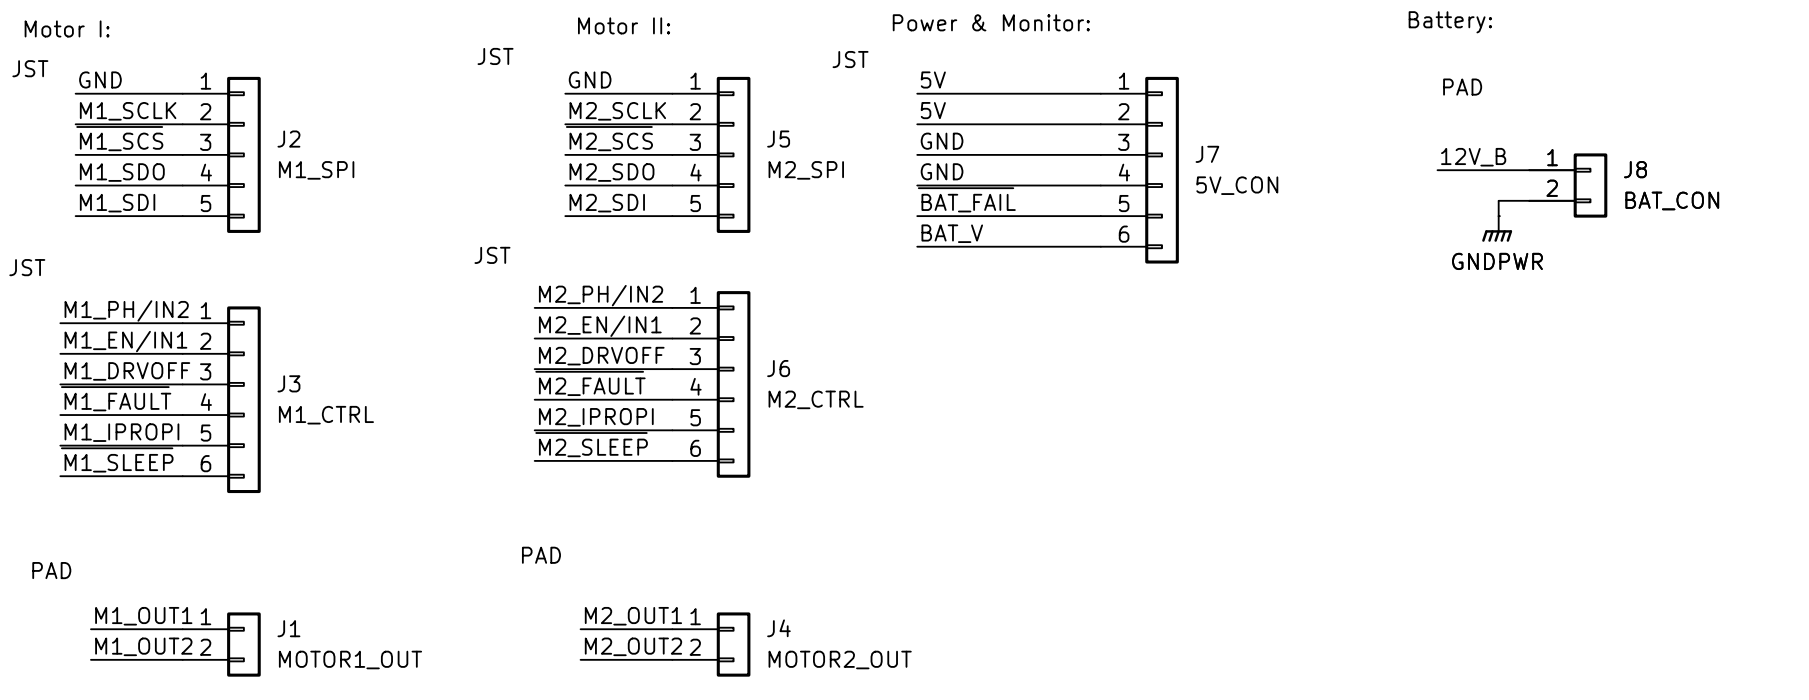
\includegraphics[width=\textwidth]{figures/Hardware/Connections_PCSU_Schematic.png}
    \caption{Teljesítményelektronikai NYÁK csatlakozói}
    \label{fig:pcsu-csatlakozok}
\end{figure}


A NYÁK elrendezésénél a gyártói 

\subsubsection{Felhasználónak visszajezlés}
A panelen 6 LED biztosít vizuális visszajelzést a felhasználó számára a tápágak és a 
motorkimenetek állapotáról.
A védett 12~V-os tápág feszültségének ellenőrzésére egy egy piros LED jelzi, 2.7~k$\Omega$-os előtét
ellenállással. A 5~V-os tápág feszültségének állapotát szintén egy piros LED jelzi, 1~k$\Omega$-os előtét ellenállással.

Mindkét motorvezérlő két kimenetéhez 1-1 sárga LED tartozik, 1 ~k$\Omega$ előtét ellenállásál. 
Ezek a motorkimenetek feszültségi állapotát jelzik a vizuálisan a felhasználó számára.  \\ 

\subsection{NYÁK elrendezése és felépítése}
A teljesítményelektronikai panel négyrétegű,  98~mm~$\times$~98~mm méretű nyomtatott áramkör.
Az alkatrészek a NYÁK felső oldalán kapnak helyet.A NYÁK 1,6~mm vastagságú FR-4 alapanyagból, TG135 anyagminőséggel. A külső rézrétegek névleges réztömege
1~oz/ft$^2$, a belső rétegeké 0,5~oz/ft$^2$. 

A rétegfelépítés és az elrendezések kialakításámál a nagyáramú tápágak, a vezérlőjelek
elvezetése és a teljesítményalkatrészek hőelvezetése voltak a fő szempontok.

\subsubsection{NYÁK rétegei}
A NYÁK rétegei a következőképpen lettek kialakítva:
\begin{itemize}
    \item \textbf{Felső rézréteg (F. Cu):} Jelréteg, ahol amelyen helyet kaptak a különböző elektronikai alkatrészek, 
    valamint a jelölések és a NYÁK-on található szöveges információk
    \item \textbf{Első belső rézréteg (In1.Cu):} Földkitöltések rétege. A szétválasztott GNDPWR a 12~V-os tápfeszültséghez tartozó földhálózat, 
    valamint a 5~V-os tápfeszültséghez tartozó földhálózat kitöltése található a rétegen. 
    \item \textbf{Második belső rézréteg (In2.Cu):} a védett 12~V-os tápfeszültség kitöltése található a rétegem 
    \item \textbf{Alsó rézréteg (B.Cu):} Alsó jelréteg. A nem használt helyeken mind a nagyteljesítményű GNDPWR földhálózat, mind a
    az 5~V-os tápfeszültség földhálózata szétválasztva található.
\end{itemize}

\begin{figure}[htbp]
    \centering
    \begin{minipage}{0.48\textwidth}
        \centering
        \includesvg[width=\linewidth,inkscapelatex=false]{figures/Hardware/Szakdolgozat_PCSU-F_Cu}
        \par\smallskip
        (a) Felső rézréteg
    \end{minipage}
    \hfill
    \begin{minipage}{0.48\textwidth}
        \centering
        \includesvg[width=\linewidth,inkscapelatex=false]{figures/Hardware/Szakdolgozat_PCSU-In1_Cu}
        \par\smallskip
        (b) Első belső rézréteg
    \end{minipage}

    \par\medskip

    \begin{minipage}{0.48\textwidth}
        \centering
        \includesvg[width=\linewidth,inkscapelatex=false]{figures/Hardware/Szakdolgozat_PCSU-In2_Cu}
        \par\smallskip
        (c) Második belső rézréteg
    \end{minipage}
    \hfill
    \begin{minipage}{0.48\textwidth}
        \centering
        \includesvg[width=\linewidth,inkscapelatex=false]{figures/Hardware/Szakdolgozat_PCSU-B_Cu}
        \par\smallskip
        (d) Alsó rézréteg
    \end{minipage}
    \caption{A teljesítményelektronikai NYÁK rézrétegei}
    \label{fig:teljesitmeny-panel-rezretegek}
\end{figure}

\subsubsection{NYÁK elrendezése}
A NYÁK elrendezésénél a fő szempont az GND hurkok elkerülése volt.

A \ref{fig:pcsu-elrendezes} ábrán látható a NYÁK elrendezése:
\begin{figure}[H]
    \centering
    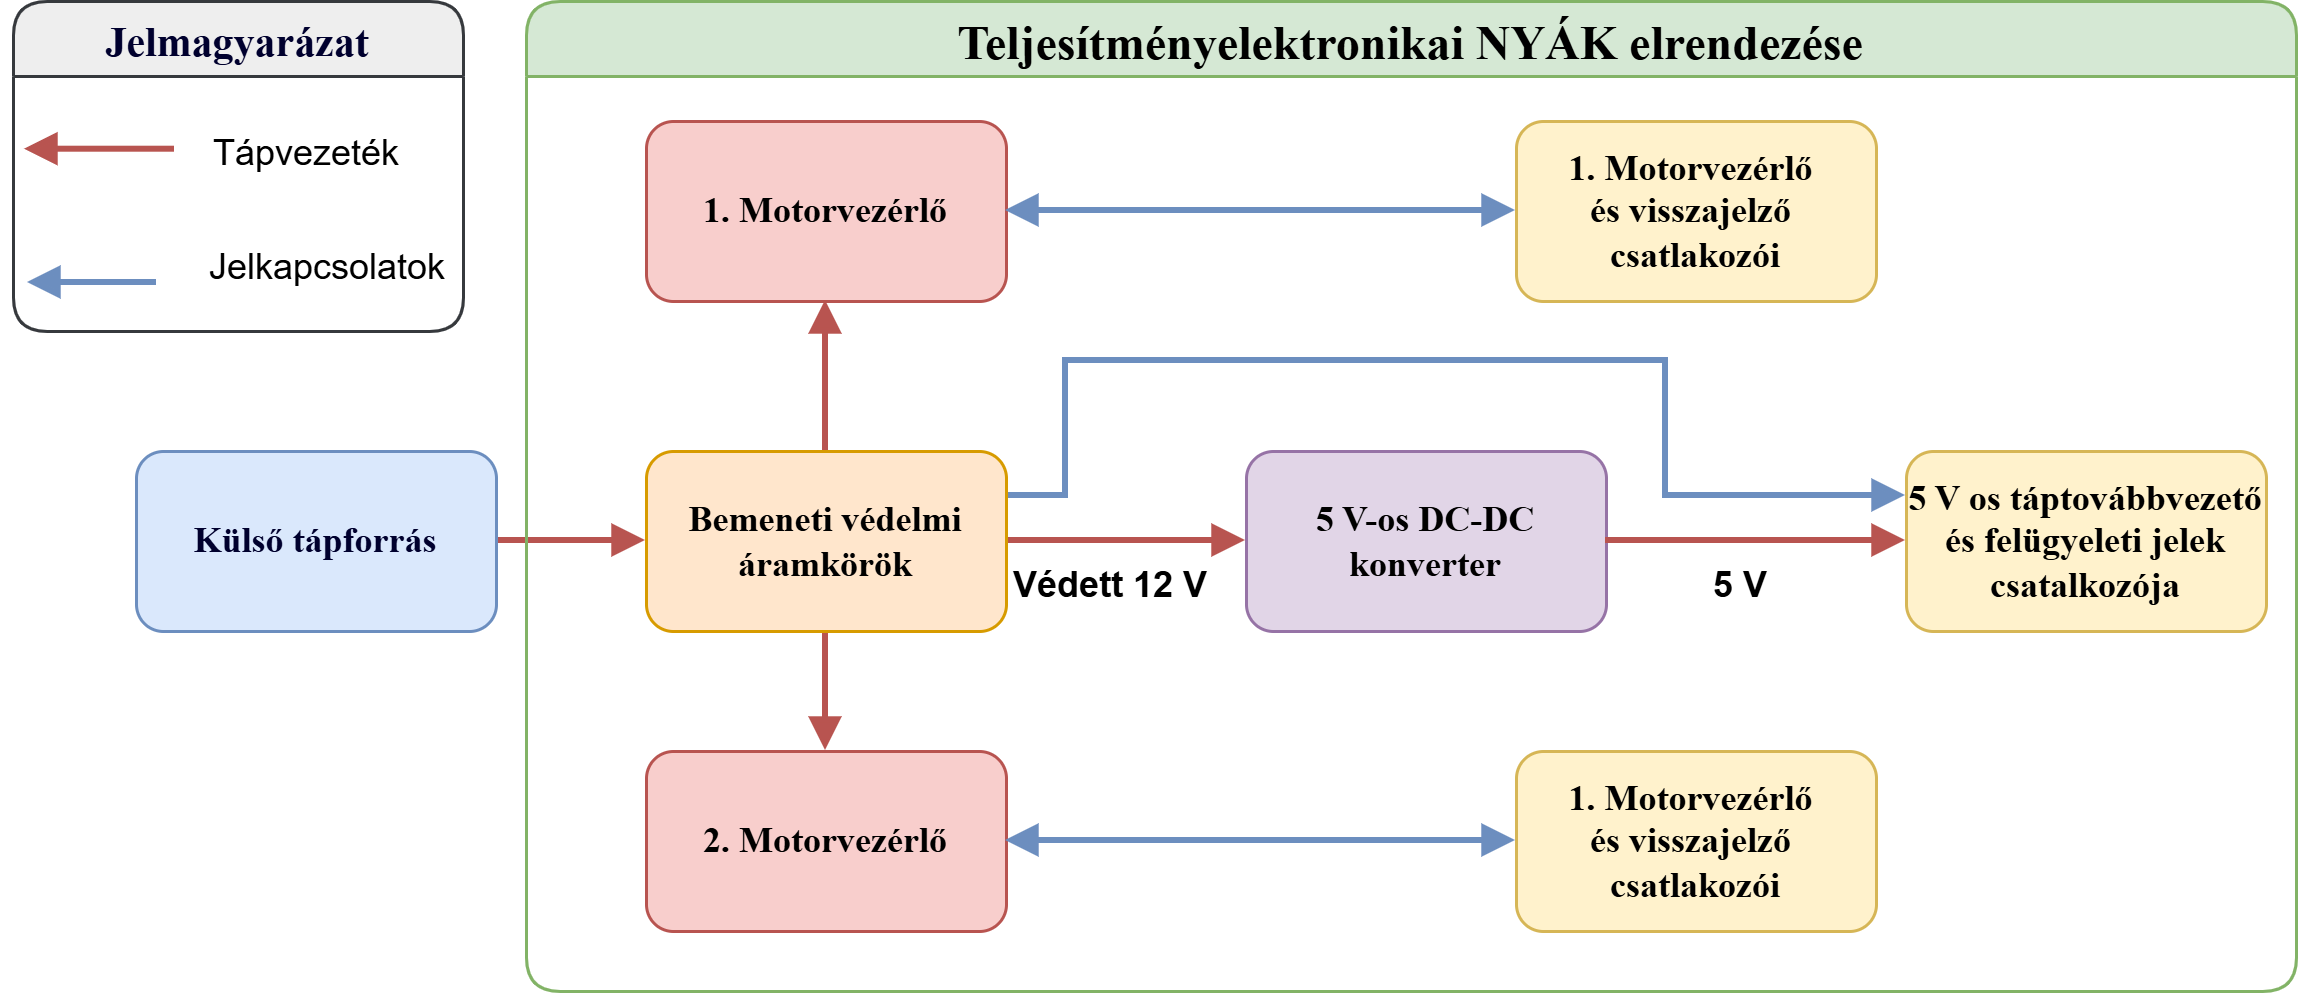
\includegraphics[width=\textwidth]{figures/Hardware/SzakdogaSystemDiagramms-PCSU_Elrendezés.drawio.png}
    \caption{Teljesítményelektronikai NYÁK elrendezése}
    \label{fig:pcsu-elrendezes}
\end{figure}

\textcolor{red}{megmutatni ezt a rendes NYÁK tervel is}



% ------------------------------------------------------------------
\section{Központi vezérlő NYÁK tervezése}
\label{sec:kozponti-vezérlő-NYAK}
% ------------------------------------------------------------------

A központi vezérlőpanel a motorok működésének vezérlését, a felhasználói
interfész kezelését, az


\subsection{Tápellátás}
A központi vezérlőpanel tápellátása 3 tápvonalon oszlik meg: 5~V-os, 5V\_System 
és a 3,3~V-os tápágra.

Az 5~V-os tápágot, a teljesítményelektronikai panelről érkező tápellátás biztosítja.
Ez az egyik forrása az 5V\_System tápágnak, biztosítja a rádiós vevőmodulok és a rácsatlakoztatható bővítő panelok tápellátását.

Az 5V\_System tápág forrása egy MUX segítségével választódik ki a teljesítményelektronikai panelről jövő 5~V-os 
tápellátás és az USB porton keresztül jövő 5~V-os tápfeszültség közül. Ez biztosítja a tápellátást a 
GPS, az IMU modulnak vmin a 3,3~V-os tápvonalat is előállító lineáris feszültségszabályzónak.

A 3,3~V-os tápág biztosítja a mikrovezérlő, a flash memória, az SD kártya és a motorenkóderek
tápellátását. Egy alternatív tápforrása a tápágnak még egy programozáskor használható 
3,3~V-ot biztosító PIN csatlakozó.

A tápágak felépítését és a hozzájuk kapcsolódó fogyasztókat a 
\ref{fig:cu-tapvonalak}.~ábra mutatja be:

\begin{figure}[H]
    \centering
    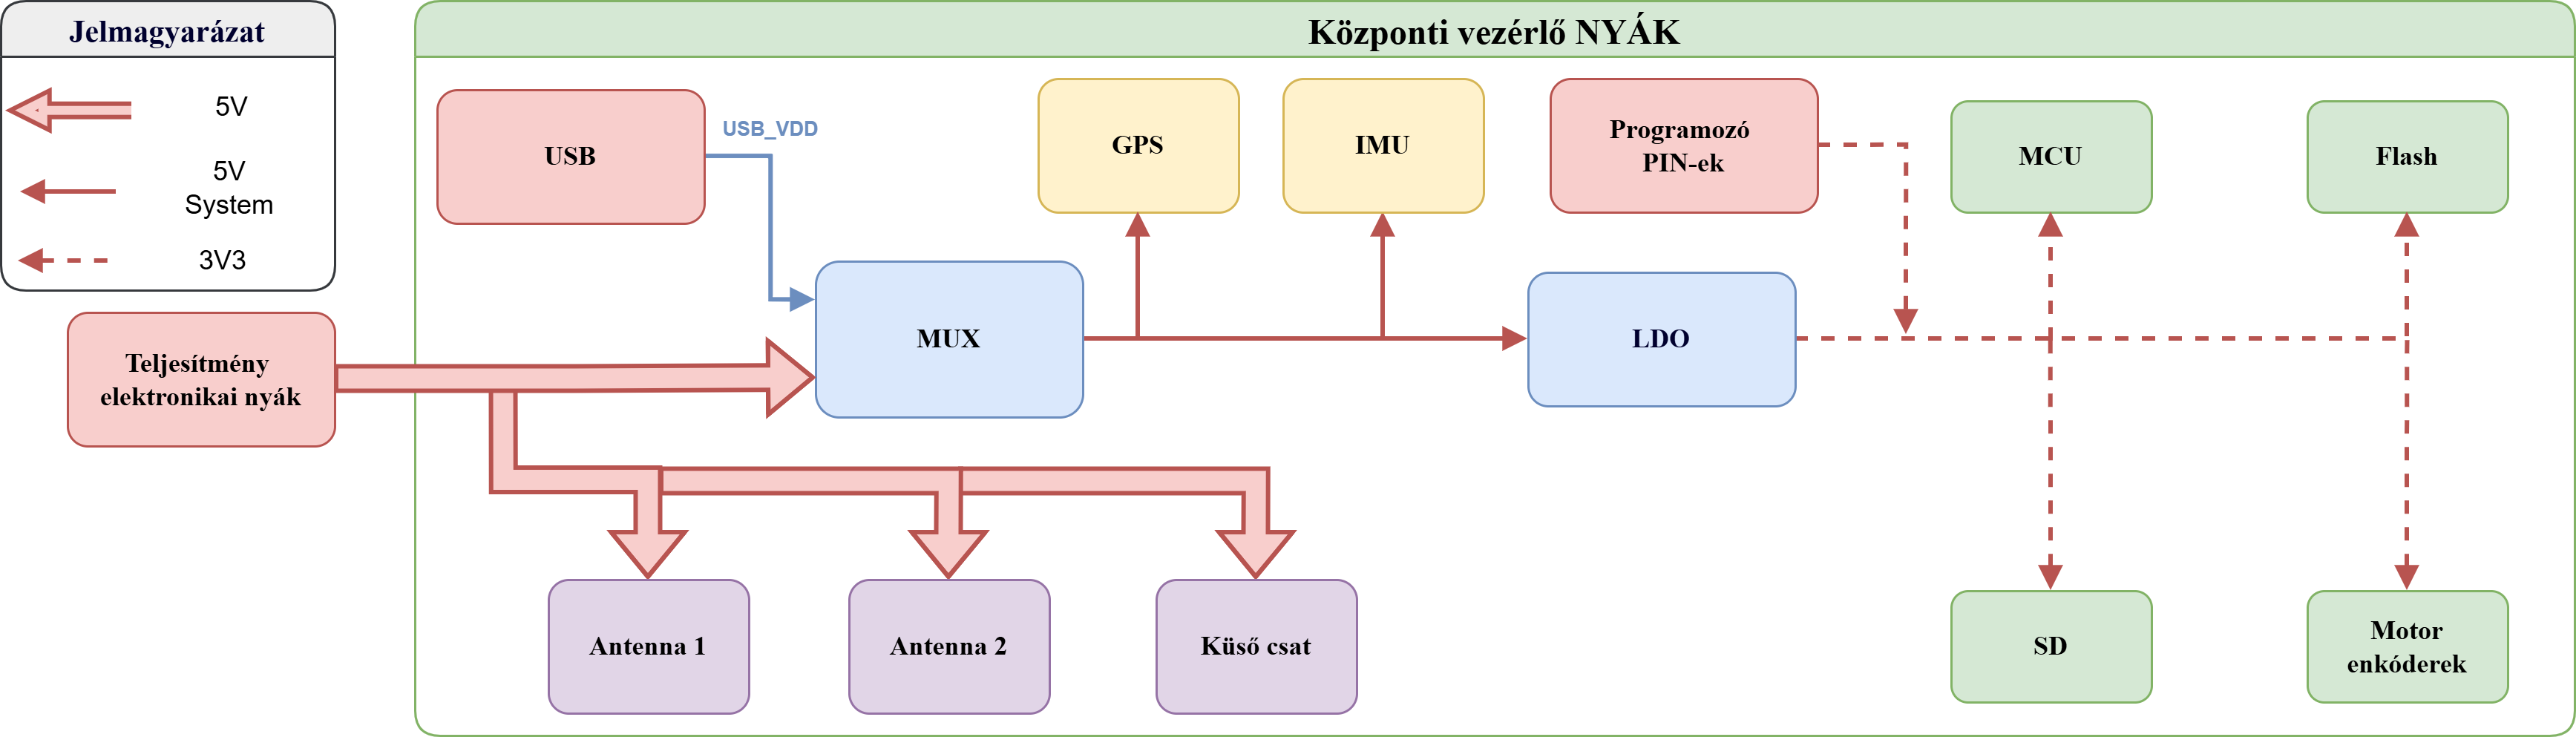
\includegraphics[width=\textwidth]{figures/Hardware/SzakdogaSystemDiagramms-CU_Tápvonalak.drawio.png}
    \caption{Központi vezérlőpanel tápvonalai és hozzájuk kapcsolódó alkatrészek}
    \label{fig:cu-tapvonalak}
\end{figure}


\subsubsection{5~V-os tápellátás és  tápág választás}
Az 5V\_System tápellátás ellátást a TPS2117 tápforrásválasztó integált áramkör
segítségével választódik ki \cite{tps2117}.
A célja, hogy a rendszer fő érzékelői tesztelhetőek legyenek a teljesítményelektronikai
panel csatlakoztatása nélkül, emellett pedig egy másodlagos tápforrást adjon a rendszernek
biztonsági okokból, ha a teljesítményelektronikai panel tápálletásáa megszűnne.

A tápforrásválasztó maximum 4~A áramot képes biztosítani, ami elegendő az 5V\_System tápág
teljes terheléséhez. \textcolor{red}{LINK}

\textcolor{red}{a vevés jelen esetben akkor sem történik meg...}

Az áramkör elsődeleges tápforrása a teljesítményelektronikai panelről érkező 5~V-os
tápfeszültség, azonban ha ennek a tápfeszültségének szintje a beállított határ alá csökken,
akkor a tápforrásválasztó automatikusan átvált az USB felőli bemenetre.

\subsubsection{3,3~V-os tápellátás}
A 3,3~V-os tápellátást a TLV75533 típusú lineáris feszültségszabályzó biztosítja \cite{tlv755p}.
Az LDO 500~mA áramot képes biztosítani, ami elegendő a 3,3~V-os tápág összes fogyasztójának
kiszolgálására. \textcolor{red}{LINK}

\textcolor{red}{visszafolyás elleni védelemhez kéne dióda...}

\subsubsection{Kapcsolási rajz}

A TLV75533 lineáris feszültségszabályo

A kiválasztott LDO külön állító ellenállások nélkül, fix 3,3~V-os kimeneti feszültséget
képes előállítani.
A bemenő és a kimenő tápágához is egy-egy 1~$\mu$F-os kerámia szűrőkondenzátor lett kapcsolva,
a gyártói adatlapban [7.1]~alfejezetben. \\

A TS2117 MODE bemenete az elsődleges, VIN1 bemenethez kapcsolódó  5~V-os tápágot 
  kapcsolva, ez határozza meg
a 

A váltást meghatározó bemeneti feszültség a PR1 lábán bemenő lábán mért feszültség alapján
határozódik meg. Amikor amikor a láb feszültsége a V\_ref refereneciafeszültség alá csökken, 
amelynek értékke 1~V [6.5 tábla], átkapcsol a VIN2 feszültségre [7.3.1~alfejezet].

Mivel az R6 értéke 47~k$\Omega$, az R7 értéke pedig 15,4~k$\Omega$ így a 
következő bemeneti feszültségszintnél történik a váltás:
\begin{equation}
    V_{\mathrm{PR1}}=V_{\mathrm{IN1}}\cdot\dfrac{R_7}{R_6+R_7}
    \label{eq:cu-mux-valtas}
\end{equation}

A \ref{eq:cu-mux-valtas} egyenletet átalakítva a váltási feszültség nagysága:
\begin{equation}
    V_{\mathrm{valt}}
    = V_{\mathrm{REF}}\frac{R_6+R_7}{R_7}
    = 1~\mathrm{V}\cdot\frac{47+15{,}4}{15{,}4}
    \approx4{,}05~\mathrm{V}.
    \label{eq:cu-mux-valtas-kuszob}
\end{equation}

A választott feszültség felett az LDO még képes biztosítani a 3,3~V-os tápellátást.
\textcolor{red}{ezt azért csekkolni}

MÉG A TÖBBI PASSZÍVnek kell indoklás...


\textcolor{red}{berakni a diodát!}

\begin{figure}[H]
    \centering
    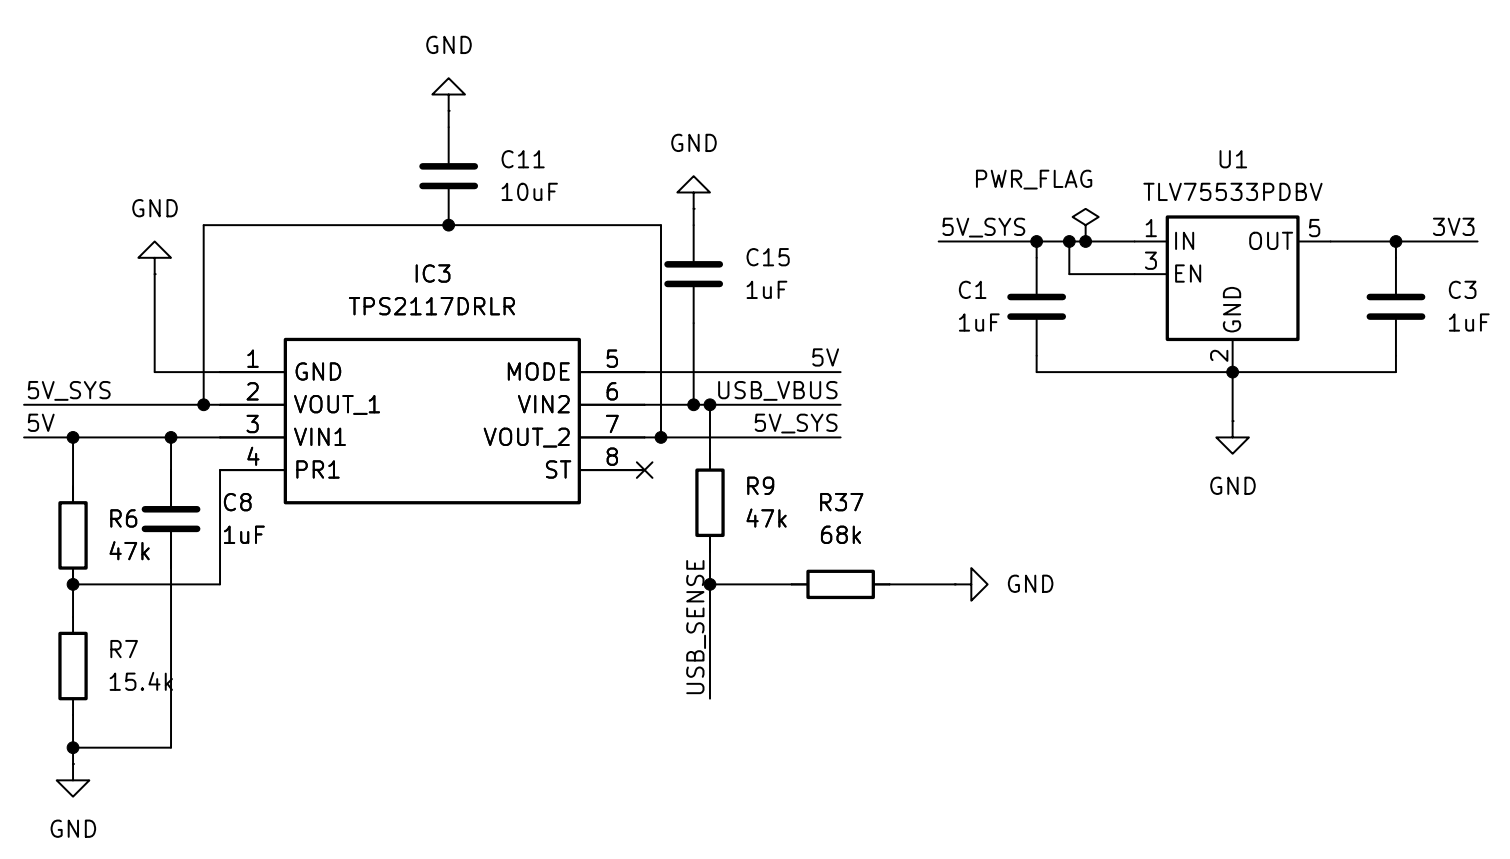
\includegraphics[width=\textwidth]{figures/Hardware/Power_Supply_CU_Schematic.png}
    \caption{Központi vezérlőpanel tápvonalanalai kapcsolási rajza}
    \label{fig:cu-tapvonalak-kapcsolasi-rajz}
\end{figure}

\subsubsection{Huzalozási terv}

\subsection{Mikrovezérlő}
A központi mikrovezérlő panel működését a \ref{subsec:mikrovez-kivalasztas} 
alfejezetben STM32F446VET6 mikrovezérlő irányítja. 

A mikrovezérlő működéséhez szükséges tápellátási, órajel-előállító,
reset és indítási áramköröket, valamint a programozási és hibakeresési interfészt
a \ref{fig:mcu-rajz}.~ábra mutatja be. \\

\begin{figure}[H]
    \centering
    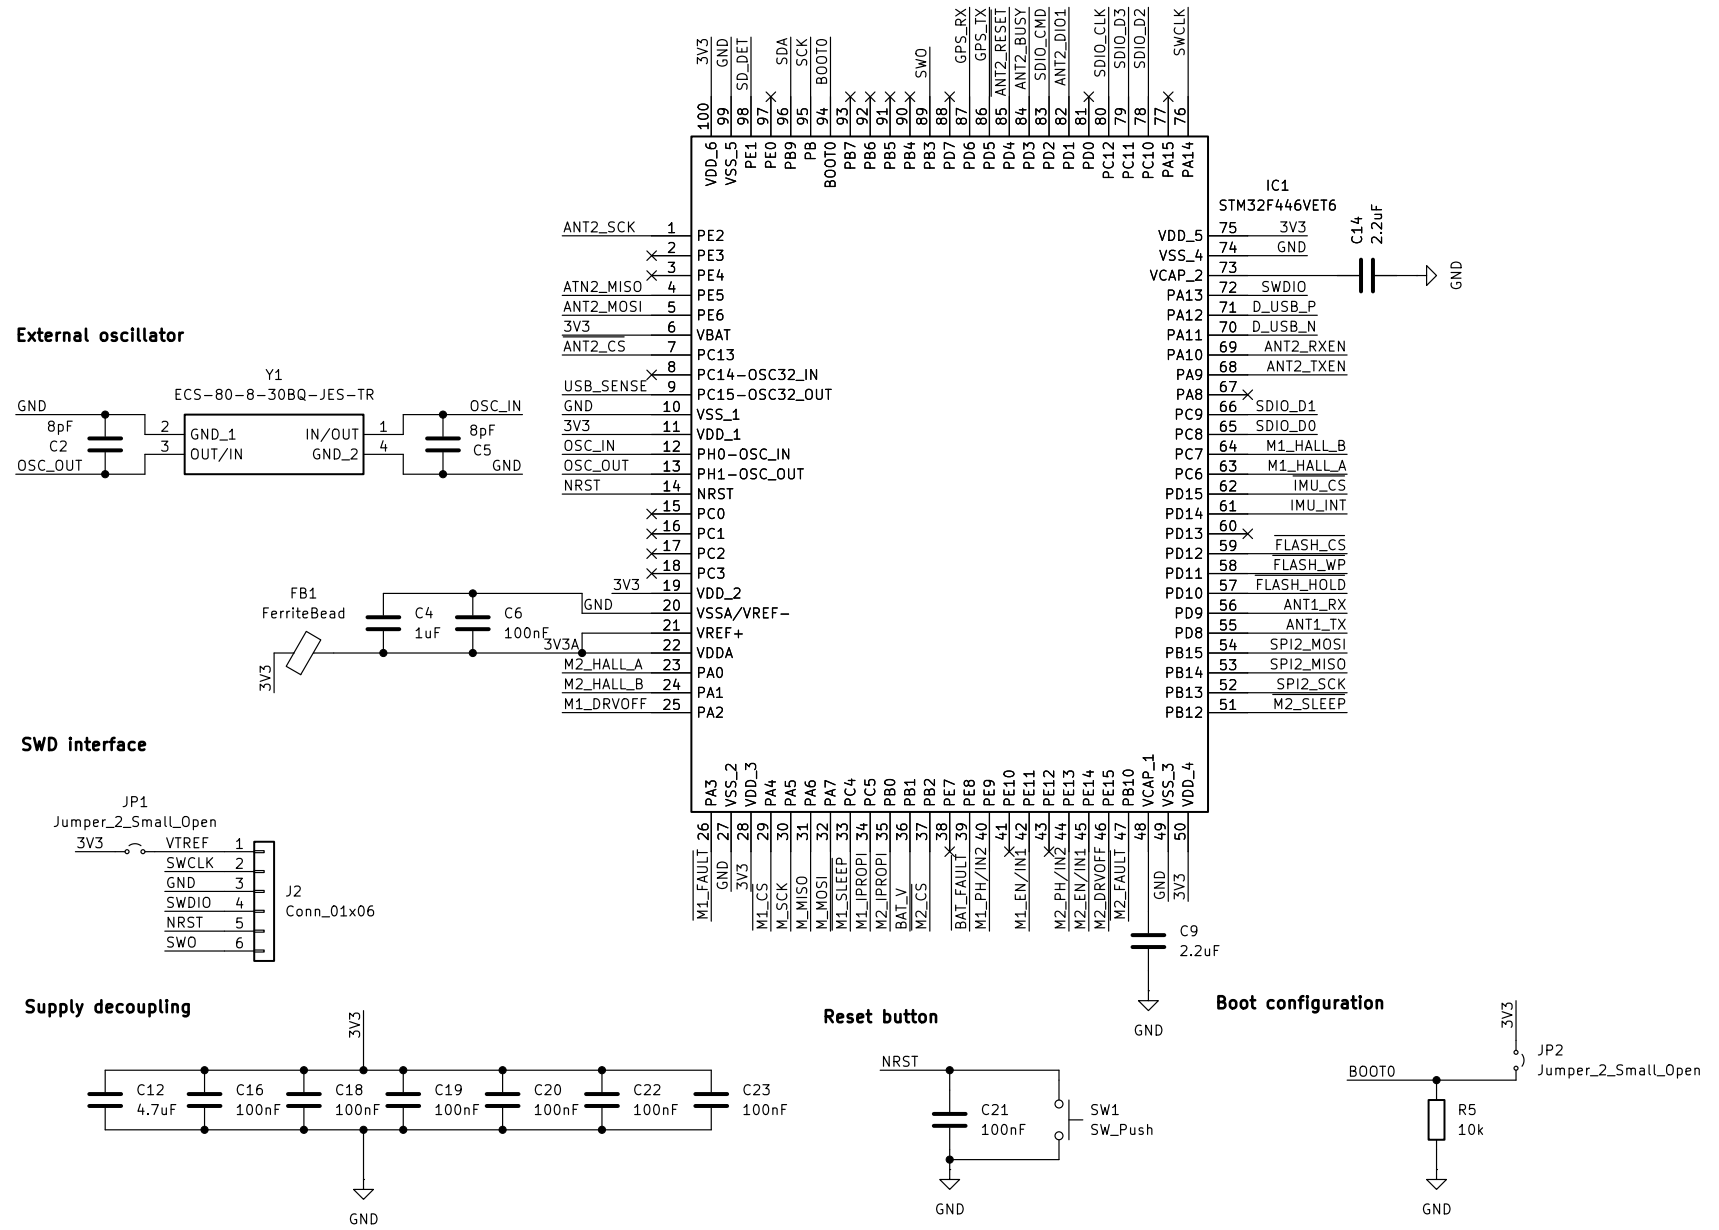
\includegraphics[width=\textwidth]{figures/Hardware/MCU_Schematic.png}
    \caption{Mikrovezérlő és hozzátartozó alkatrészek kapcsolási rajza}
    \label{fig:mcu-rajz}
\end{figure}

\subsubsection{Táp és analóg szűrőkondenzátorok}
A mirovezérlő tápellátásához tartozó kondenzátorokat
a gyártói adatlap ajánlása alapján lettek kiválasztva\cite{stm32f446re}.
A digitális tápág szűrését 100~nF-os kerámia kondenzátorok biztosítják, 
tápbemenetenként egy-egy. Ezeket egy 4,7~$\mu$F-os pufferkerámia egésziti ki.

A belső feszültségszabályzó stabil működéséhez a VCAP1 és VCAP2 kivezetésekhez egy-egy 
2,2~$\mu$F-os alacsony  ESR-ű kerámia kondenzátorok lettek kapcsolva.

Az ő analóg tápágának ellátása a 3,3~V-os tápághoz kapcsolódik egy ferrit
gyönggyön keresztül. Emellett a megfelelő
szűrés érdekében VDDA és VREF+ kapcsolodó tápág és a VSSA/VREF- között 100~nF-os és 1~$\mu$F-os 
kondenzátorok lettek elhelyezve.  

\subsubsection{Külső kristály osszilátor}
A mikrovezérlőben az USB kommunikációhoz szükséges48~MHz-es órajel előállításához
egy külső kristály szükséges. 

A kiválasztott ECS-80-8-30BQ-JES-TR kvarckristály névleges terhelőkapacitása
$C_L = 8$~pF~\cite{ecx-53bq}.

A mikrovezérlő lábának átlagos kapacitása $C_{L,MCU} = 5$~pF, 
így a szükséges kondenzátorok értéke a következőképpen számolható:
\begin{equation}
    C_{2} = C_{5} = 2\cdot(C_L) - C_{L,MCU}) = 2*8-5~\mathrm{pF} = 11~\mathrm{pF}.
    \label{eq:cu-kristaly-terhelo}
\end{equation}
Így a kristályhoz tartozó C2 és C5 kondenzátorok értéke 11~pF lett kiválasztva.
\textcolor{red}{itt 8 pF van amikor 11 kellett vna}

\subsubsection{Programozó interfész}
A programizó interfésze a mikrovezérlőnek az STM32 SWD (Serial Wire Debug) protokollját használja,
amely 2 vezetékkel egy Serial Wire Data (SWDIO) és egy Serial Wire Clock (SWCLK) vezetékkel kommunikál a programozóval.
Emellett az SWO bemenettel képes a fejlesztői környezet számára adattobabbításra. 
Ezek egy 6 pines 2.54~mm-es pinsorozatba vannak kivezetve ahol helyet kap még egy
RESET bemenet, egy föld amely összeköti a programozó földjével.
Az utolsó láb a programozáshoz szükséges 3,3~V-os tápellátást biztosítja az STM32 száméra.
Azonban ez csakis programozásra használható, emiatt egy jumper segítségével köthető be a 3,3~V-ps
tápágba. 

\subsubsection{Boot és Reset}
A mikrovezérlő kézi alaphelyzetbe állításhoz a NYÁK-on az aktív NRESET lábának alacsony szintre húzásával
érhető el. A RESET gomb a mikrovezérlő bemenetét földeli lenyomáskor, így biztosítva a hardveres
újraindítást. A RESET gombbal párhuzamosa kötött C21-es 100~nF-os kondenzátor a resetvonal
zajérzékelését csökkenti, elkerülve a folyamatos újraindítást. 

Az indítási mód kiválasztásához a BOOT0 lábához kapcsolodó jumper teszi lehetővé. 
NYitott jumper esetén az R5 10~k$\Omega$ lehúzóellenállása a BOOT0 lábát alacsony szinten
tartja így a mikrovezérlő normál üzenmódban a beégetett felhasználói programot indítja el.
A jumper zárt állapotában a BOOT1 bemenetre 3,3~V-ra kapcsolható, így a mikrovezérlő
a rendszermemóriában található gyári bootloadert indítja el, amely lehetővé teszi a 
a flash memória programozását más kommunikációs interfészek, például UART vagy USB segítségével.

\textcolor{red}{A jelenlegi kapcsolásban a PB2/BOOT1
bemenet nincs bekötve. A gyári bootloader megbízható
kiválasztásához a bemenet alacsony szintjét biztosítani
kell, például 10~k$\Omega$-os lehúzóellenállással.}

\subsection{USB csatlakozó}
A felhasznalói kommunikáció a NYÁK-on USB-C csatlakozón keresztül történik.

Az USB csatlakozóhoz egy védő integrált dióda áramkör lett kapcsolva \cite{usblc6}
A dióda engedélyezi a normál működéshez szükséges USB kommunikációt, és védi a mikrovezérlőt
a túlfeszültségtől, amely az USB csatlakozón keresztül érkezhet.

\subsubsection{Kapcsolási rajz}



\begin{figure}[H]
    \centering
    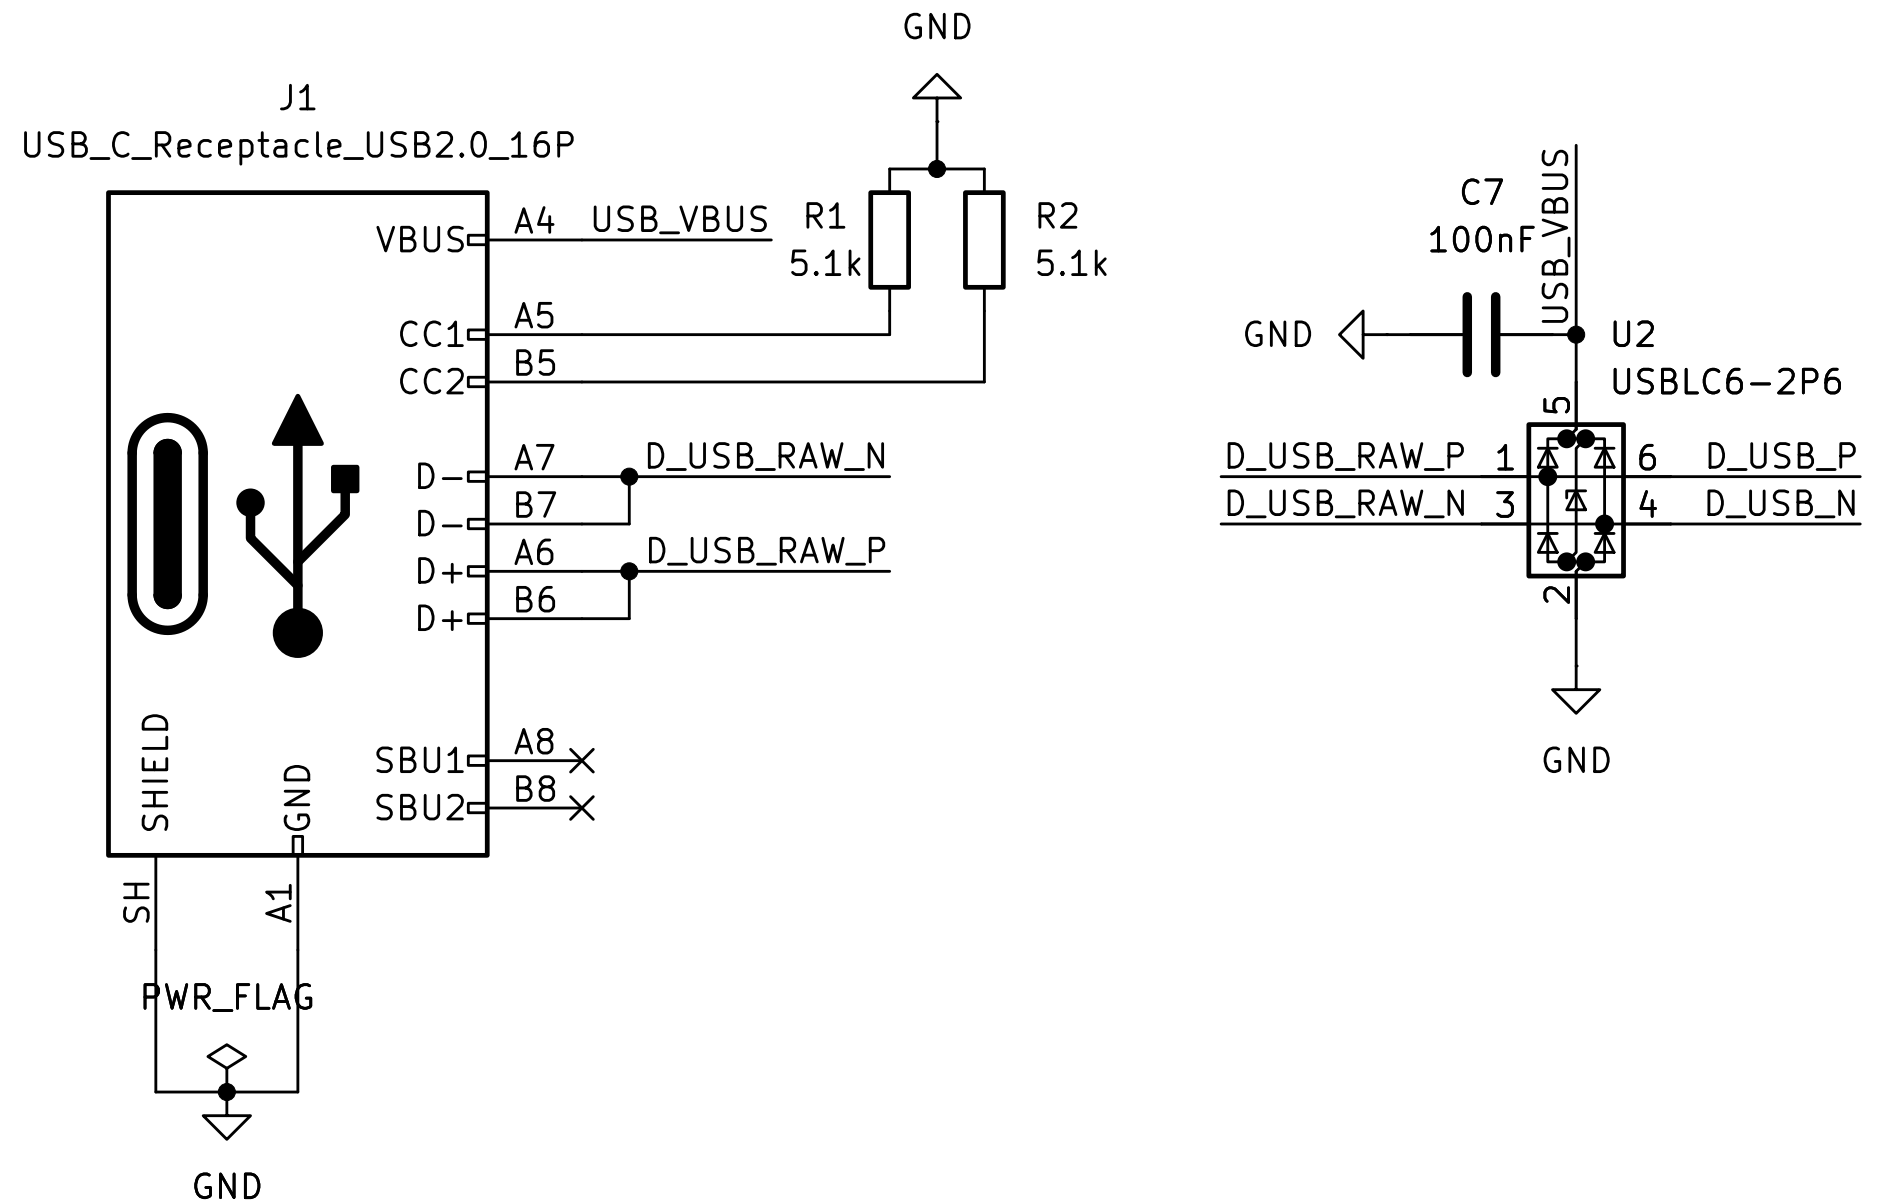
\includegraphics[width=\textwidth]{figures/Hardware/USB_CU_Schematic.png}
    \caption{Központi vezérlőpanel USB csatlakozóhoz tartozó kapcsolási rajza}
    \label{fig:mcu-rajz}
\end{figure}

\subsubsection{Huzalozási terv}
\textcolor{red}{Sztem ez nem szukseges}

\subsection{Adattárolás}

A központi vezérlőpanelen egy beépített flash memória és egy microSD kártya biztosítja
az adattárolást. 

\textcolor{red}{Flash - kalibrációs adatok, vészhelyzeti adatok; SD kartya - 
motorok és a GPS adatok, IMU adatok, stb. + telemetrian kapott adatok?}

\subsubsection{Flash memória}
A beépített adattároláshoz  W25Q256JVEIM típusú, SPI interfészes NOR flash
lett használva \cite{w25q256jv}.
A flash 256~M-bit kapacitású, és az írási és olvasási műveletekhez .... 
sebességgel rendelkezik.

\subsubsection{SD kártya}
A nagy memóriás, kivehető microSD kártya 4 bites SDIO kommunikációs protokollal
lett bekötve, amely lehetővé teszi az adatok gyors, párhuzamos átvitelét. 
A kártya eltávolítása lehetővé teszi a felhasználó számár az adatok
egyszerű kiolvasását és feldolgozását számítógépen.

\textcolor{red}{rovidek a fejezet ezt a 3-at egybe rakni?}


\subsubsection{Kapcsolási rajz}

A flash memóriának aktív alacsony CS, WP és HOLD bemeneteihez tartozó 
felhuzó ellenállásokhoz, a 10 k$\Omega$-os ellenállások lettek implementálva, 
míg a tápbemehetéhez egy 100~nF-os kerámia lett kapcsolva a zajcsökkentés érdekében. \\

Az microSD kártya csatlakozása, az alábbi cikk szolgál alapként \cite{sdcard-source}.
A csatlakozásához az DAT0--DAT3 adatvonalok és a CMD parancsvonal 47 k$\Omega$-os 
felhúzóellenálássálokkal keresztül lettek bekötve a 3.3~os tápághoz. 
A CLK órajelvonalhoz 33~$\Omega$-os csillapító soros ellenállás lett kapcsolva.
A bemenő tápvonalhoz egy 100~nF és egy 10~$\mu$F-os kerámia szűrőkondenzátor 
lett kapcsolva.

A kártya jelenlétének érzékelésére a csatlakozó mechanikus érzékelőkapcsolója szolgál.
A kártyadetektáló kimenetek közül az egyik GND-re lett húzva, míg a másik
SD\_DET jelvezetéken  jelzi a kártya jelenlétét. A jel magasra húzását egy 10 k$\Omega$-os felhúzó
ellenállás biztosítja. \\

\begin{figure}[H]
    \centering
    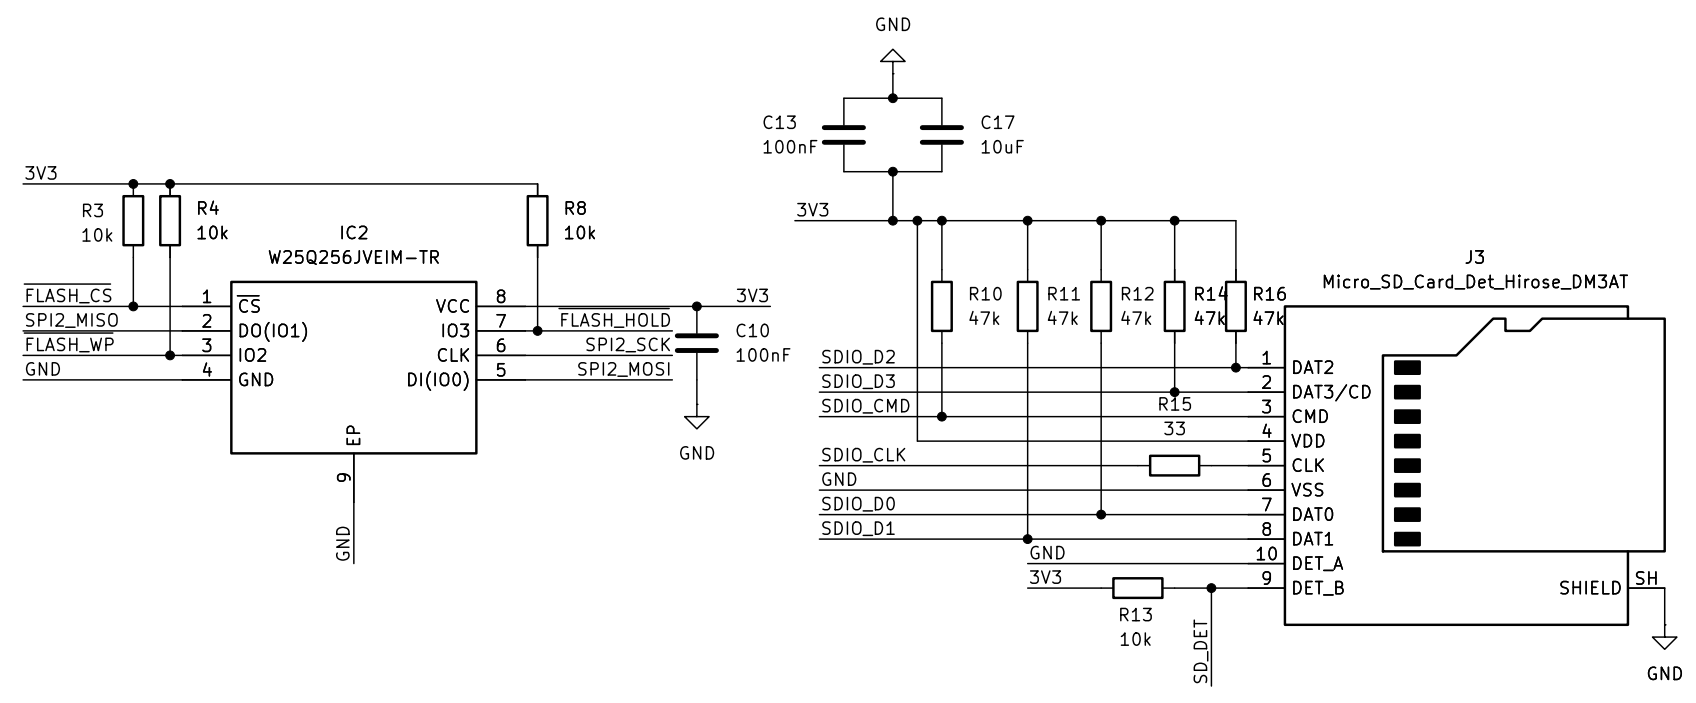
\includegraphics[width=\textwidth]{figures/Hardware/Storage_CU_Schematic.png}
    \caption{Központi vezérlőpanel adattároló egységeinek kapcsolási rajza}
    \label{fig:mcu-rajz}
\end{figure}
\subsubsection{Huzalozási terv}
\textcolor{red}{kell ez egyaltalan?}


\subsection{Csatlakozók és elrendezéseik}


\subsection{NYÁK elrendezés és huzalozás}

\section{Beültés és élesztés}
